\part{The-Unit-Step-Function}
\lecture{The Unit Step Function}{The-Unit-Step-Function}
\section{The Unit Step Function}

\title{Ordinary Differential Equations}
\subtitle{The Unit Step Function}
\date{4 November 2013}

\begin{frame}
  \titlepage
\end{frame}

\begin{frame}
  \frametitle{Outline}
  \tableofcontents[ currentsection ]
\end{frame}


\subsection{The Unit Step Function}


\begin{frame}
  \frametitle{Wouldn't it be nice....}

  \centerline{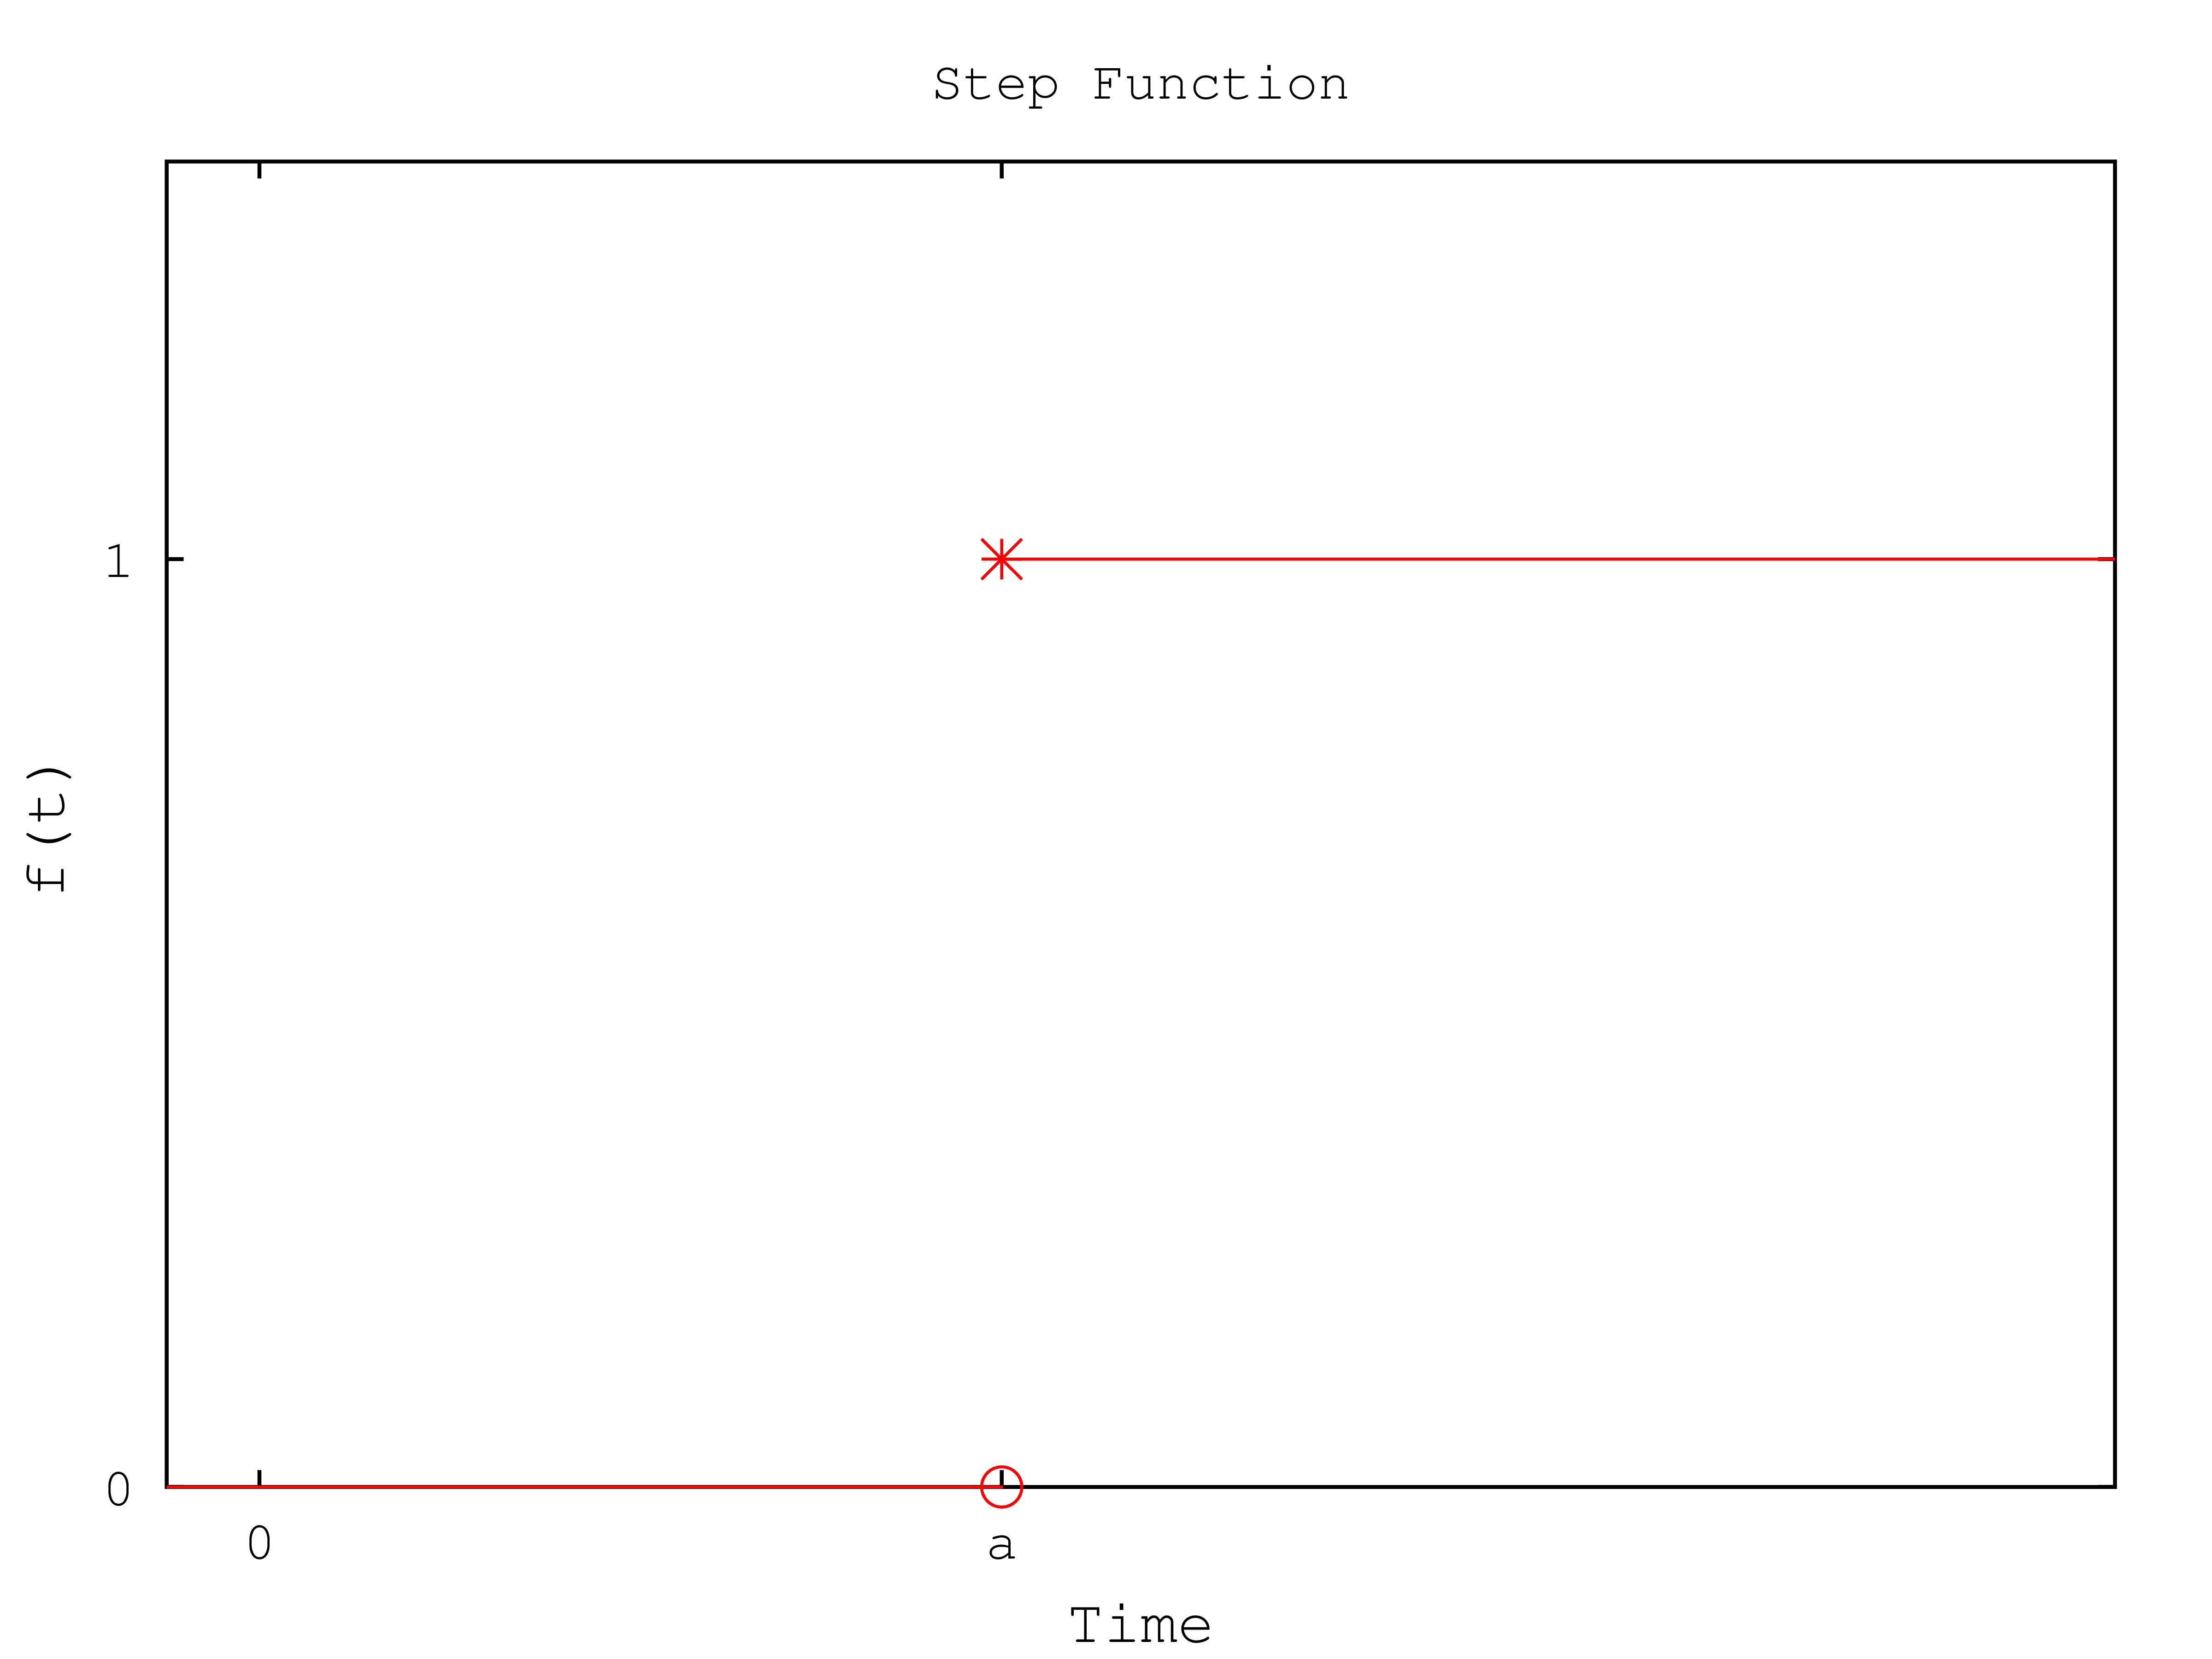
\includegraphics[width=5cm]{img/unitStepAta}}

  \uncover<2->
  {%

    Despite what you may have heard, nature is not continuous, and it
    is not differentiable.  In mechanical systems switches flip on and
    off, and things break. A function like this could be used to
    describe piecewise defined functions and help us deal with
    discontinuous functions. (We will see how later.)

  }

\end{frame}

\begin{frame}
  \frametitle{First...}


  \begin{columns}
  
    \column{.5\textwidth}
    If I am given $f(t)$....\\ [1.8em]
    \centerline{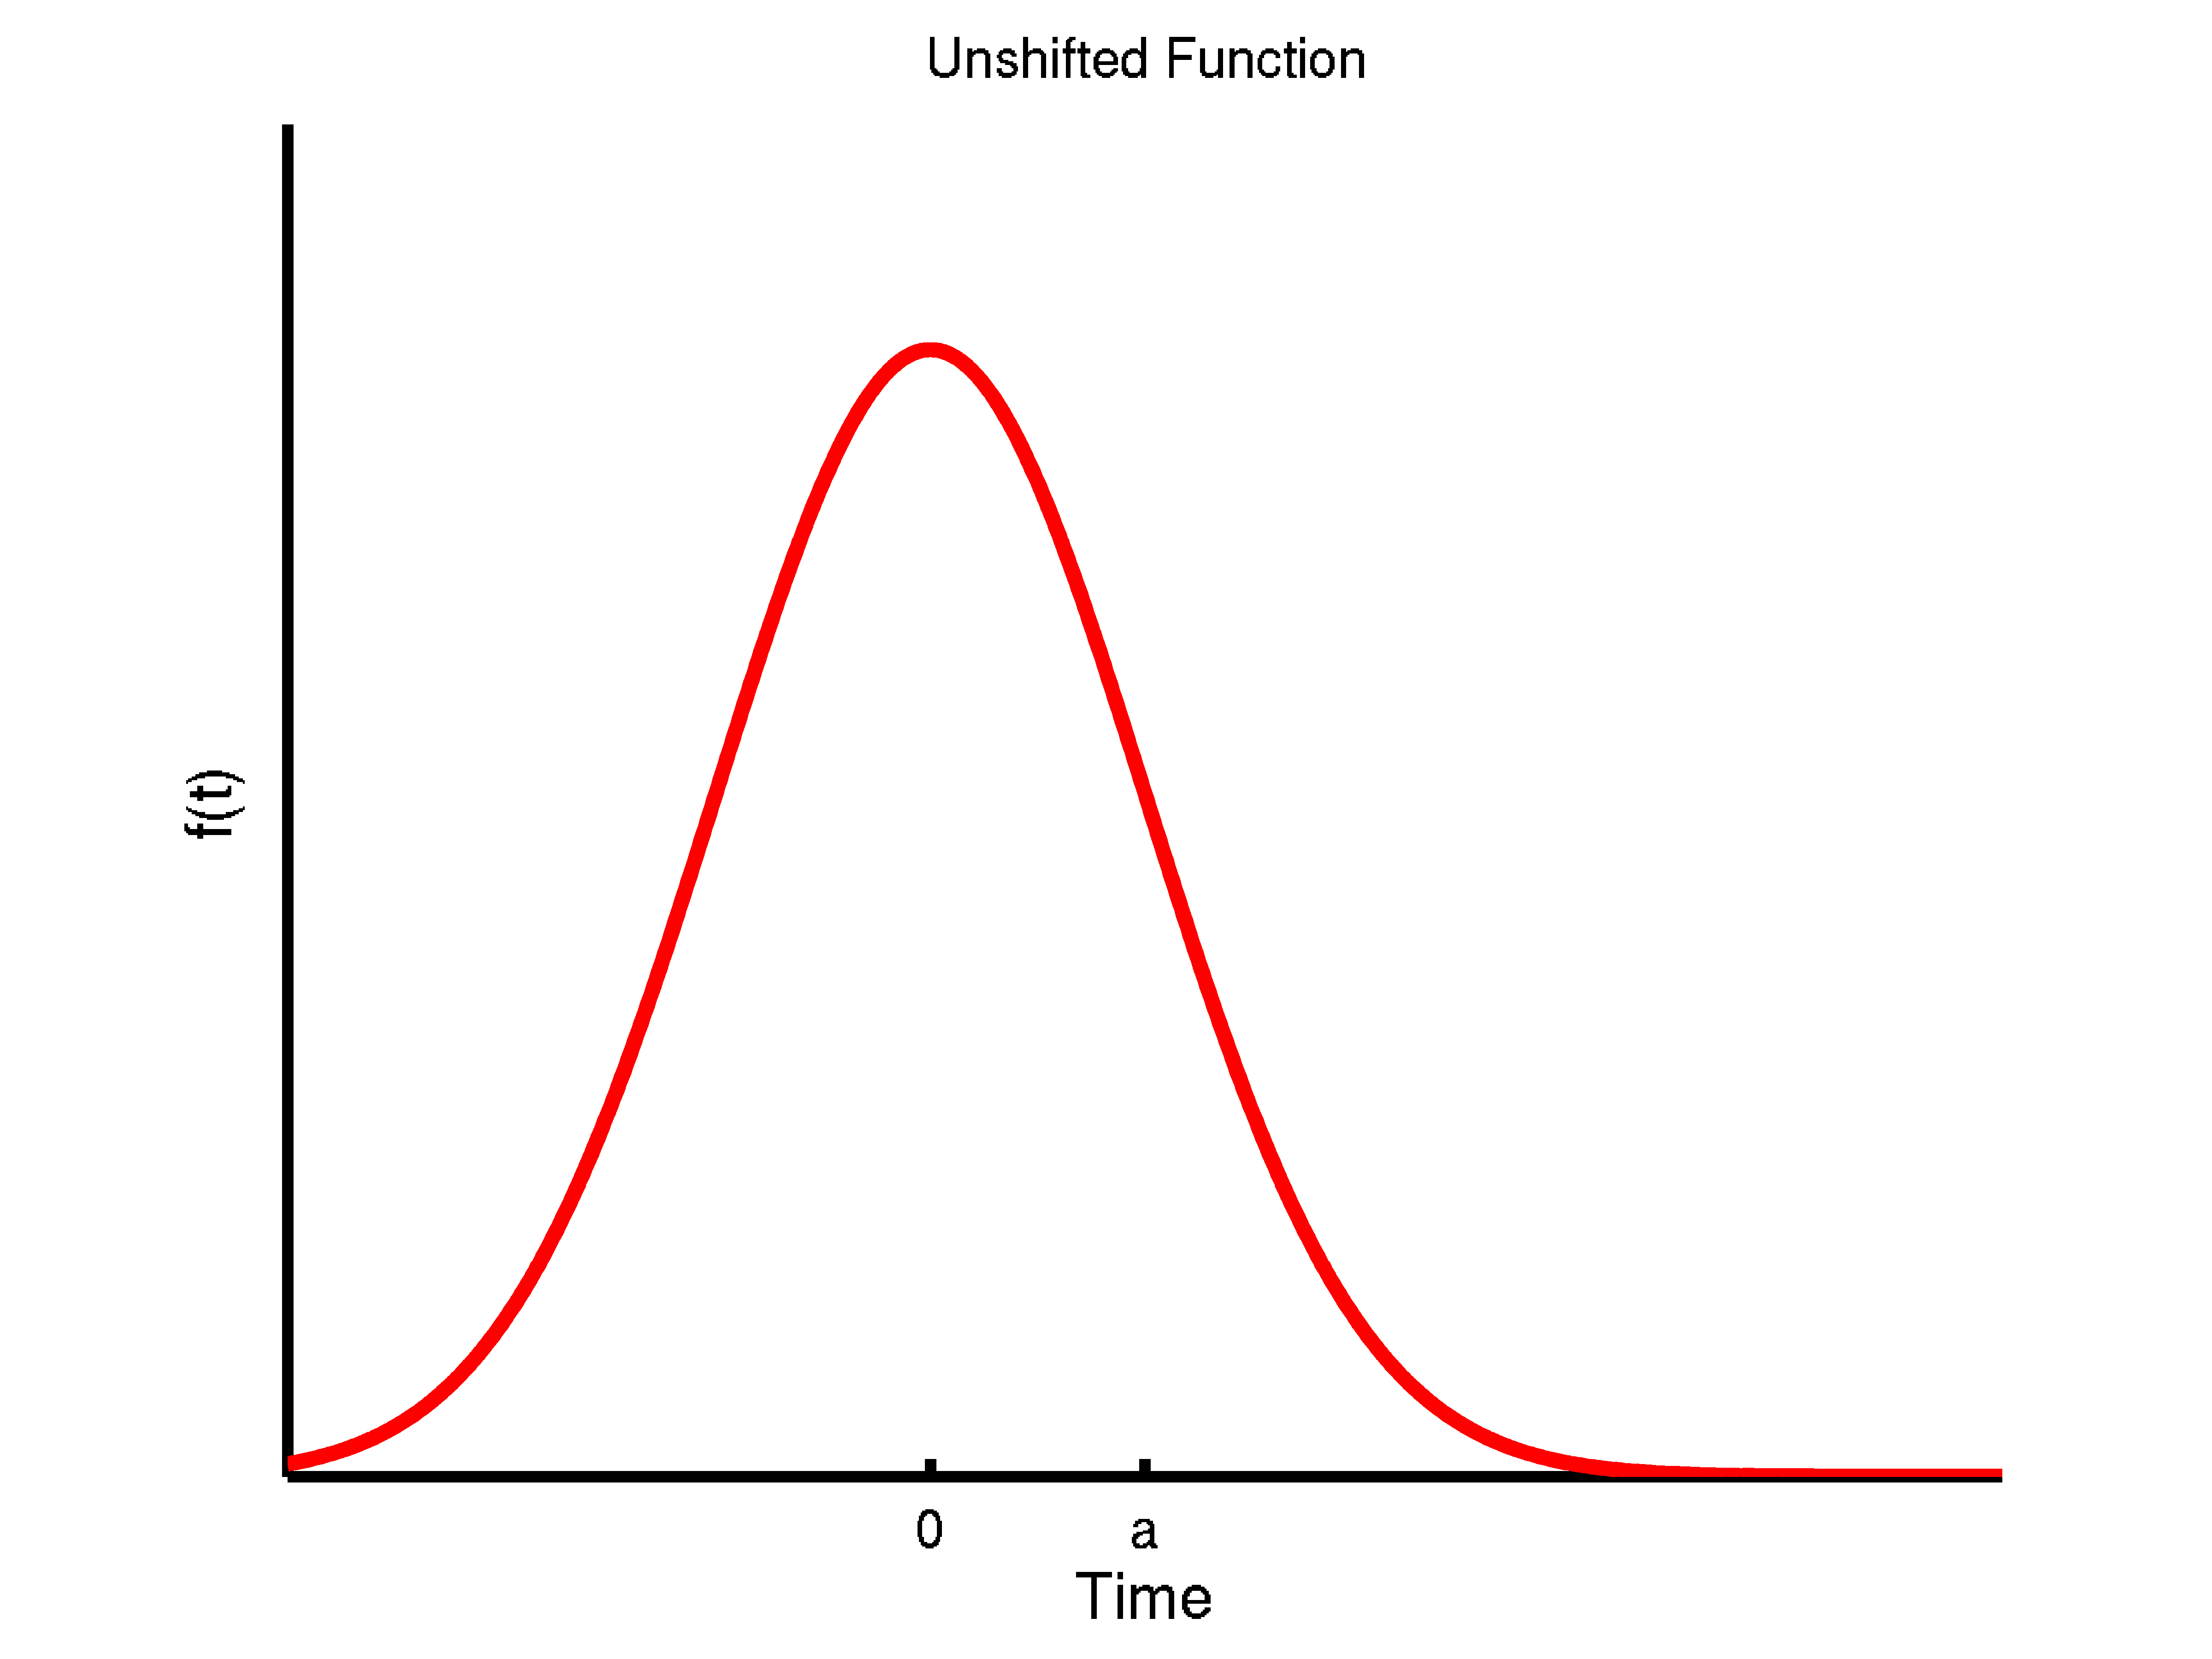
\includegraphics[width=6cm]{img/unshifted}}

    \column{.5\textwidth}
    \uncover<2->
    {%

      I can shift it to the right by translating the domain, $f(t-a)$:\\
      \centerline{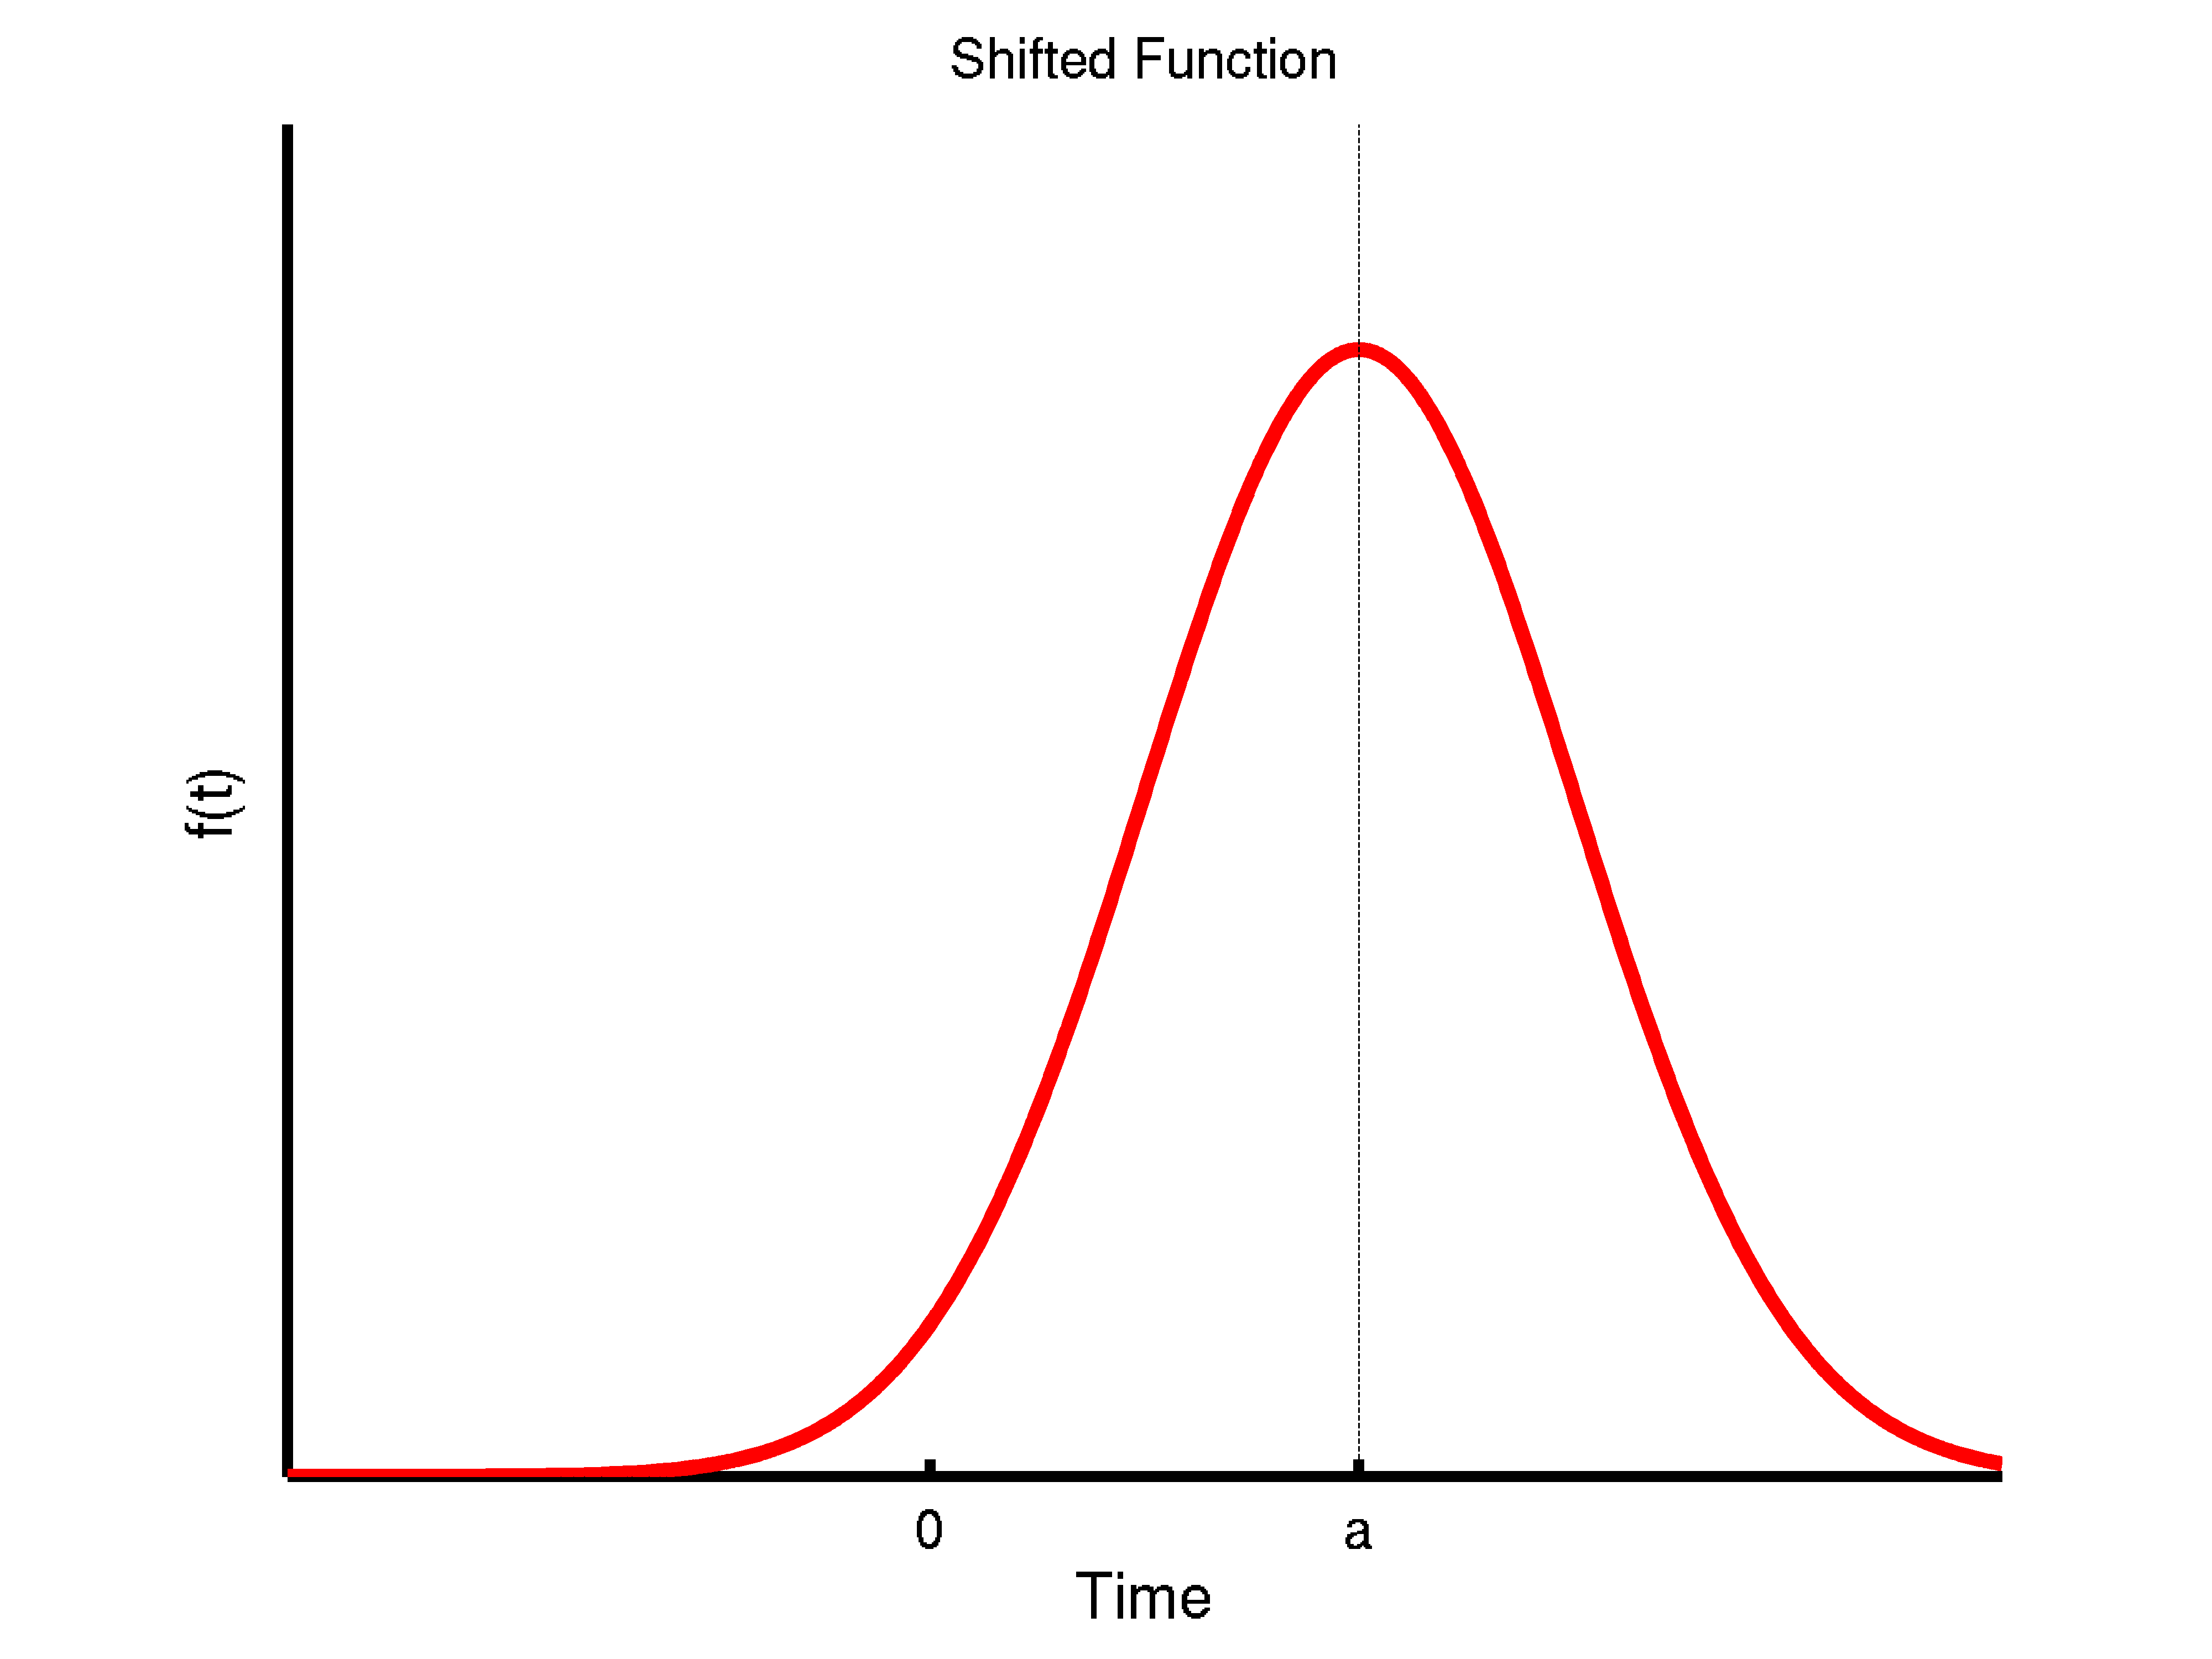
\includegraphics[width=6cm]{img/shifted}}

    }

  \end{columns}
  

\end{frame}

\begin{frame}
  \frametitle{The Unit Step Function}

  \centerline{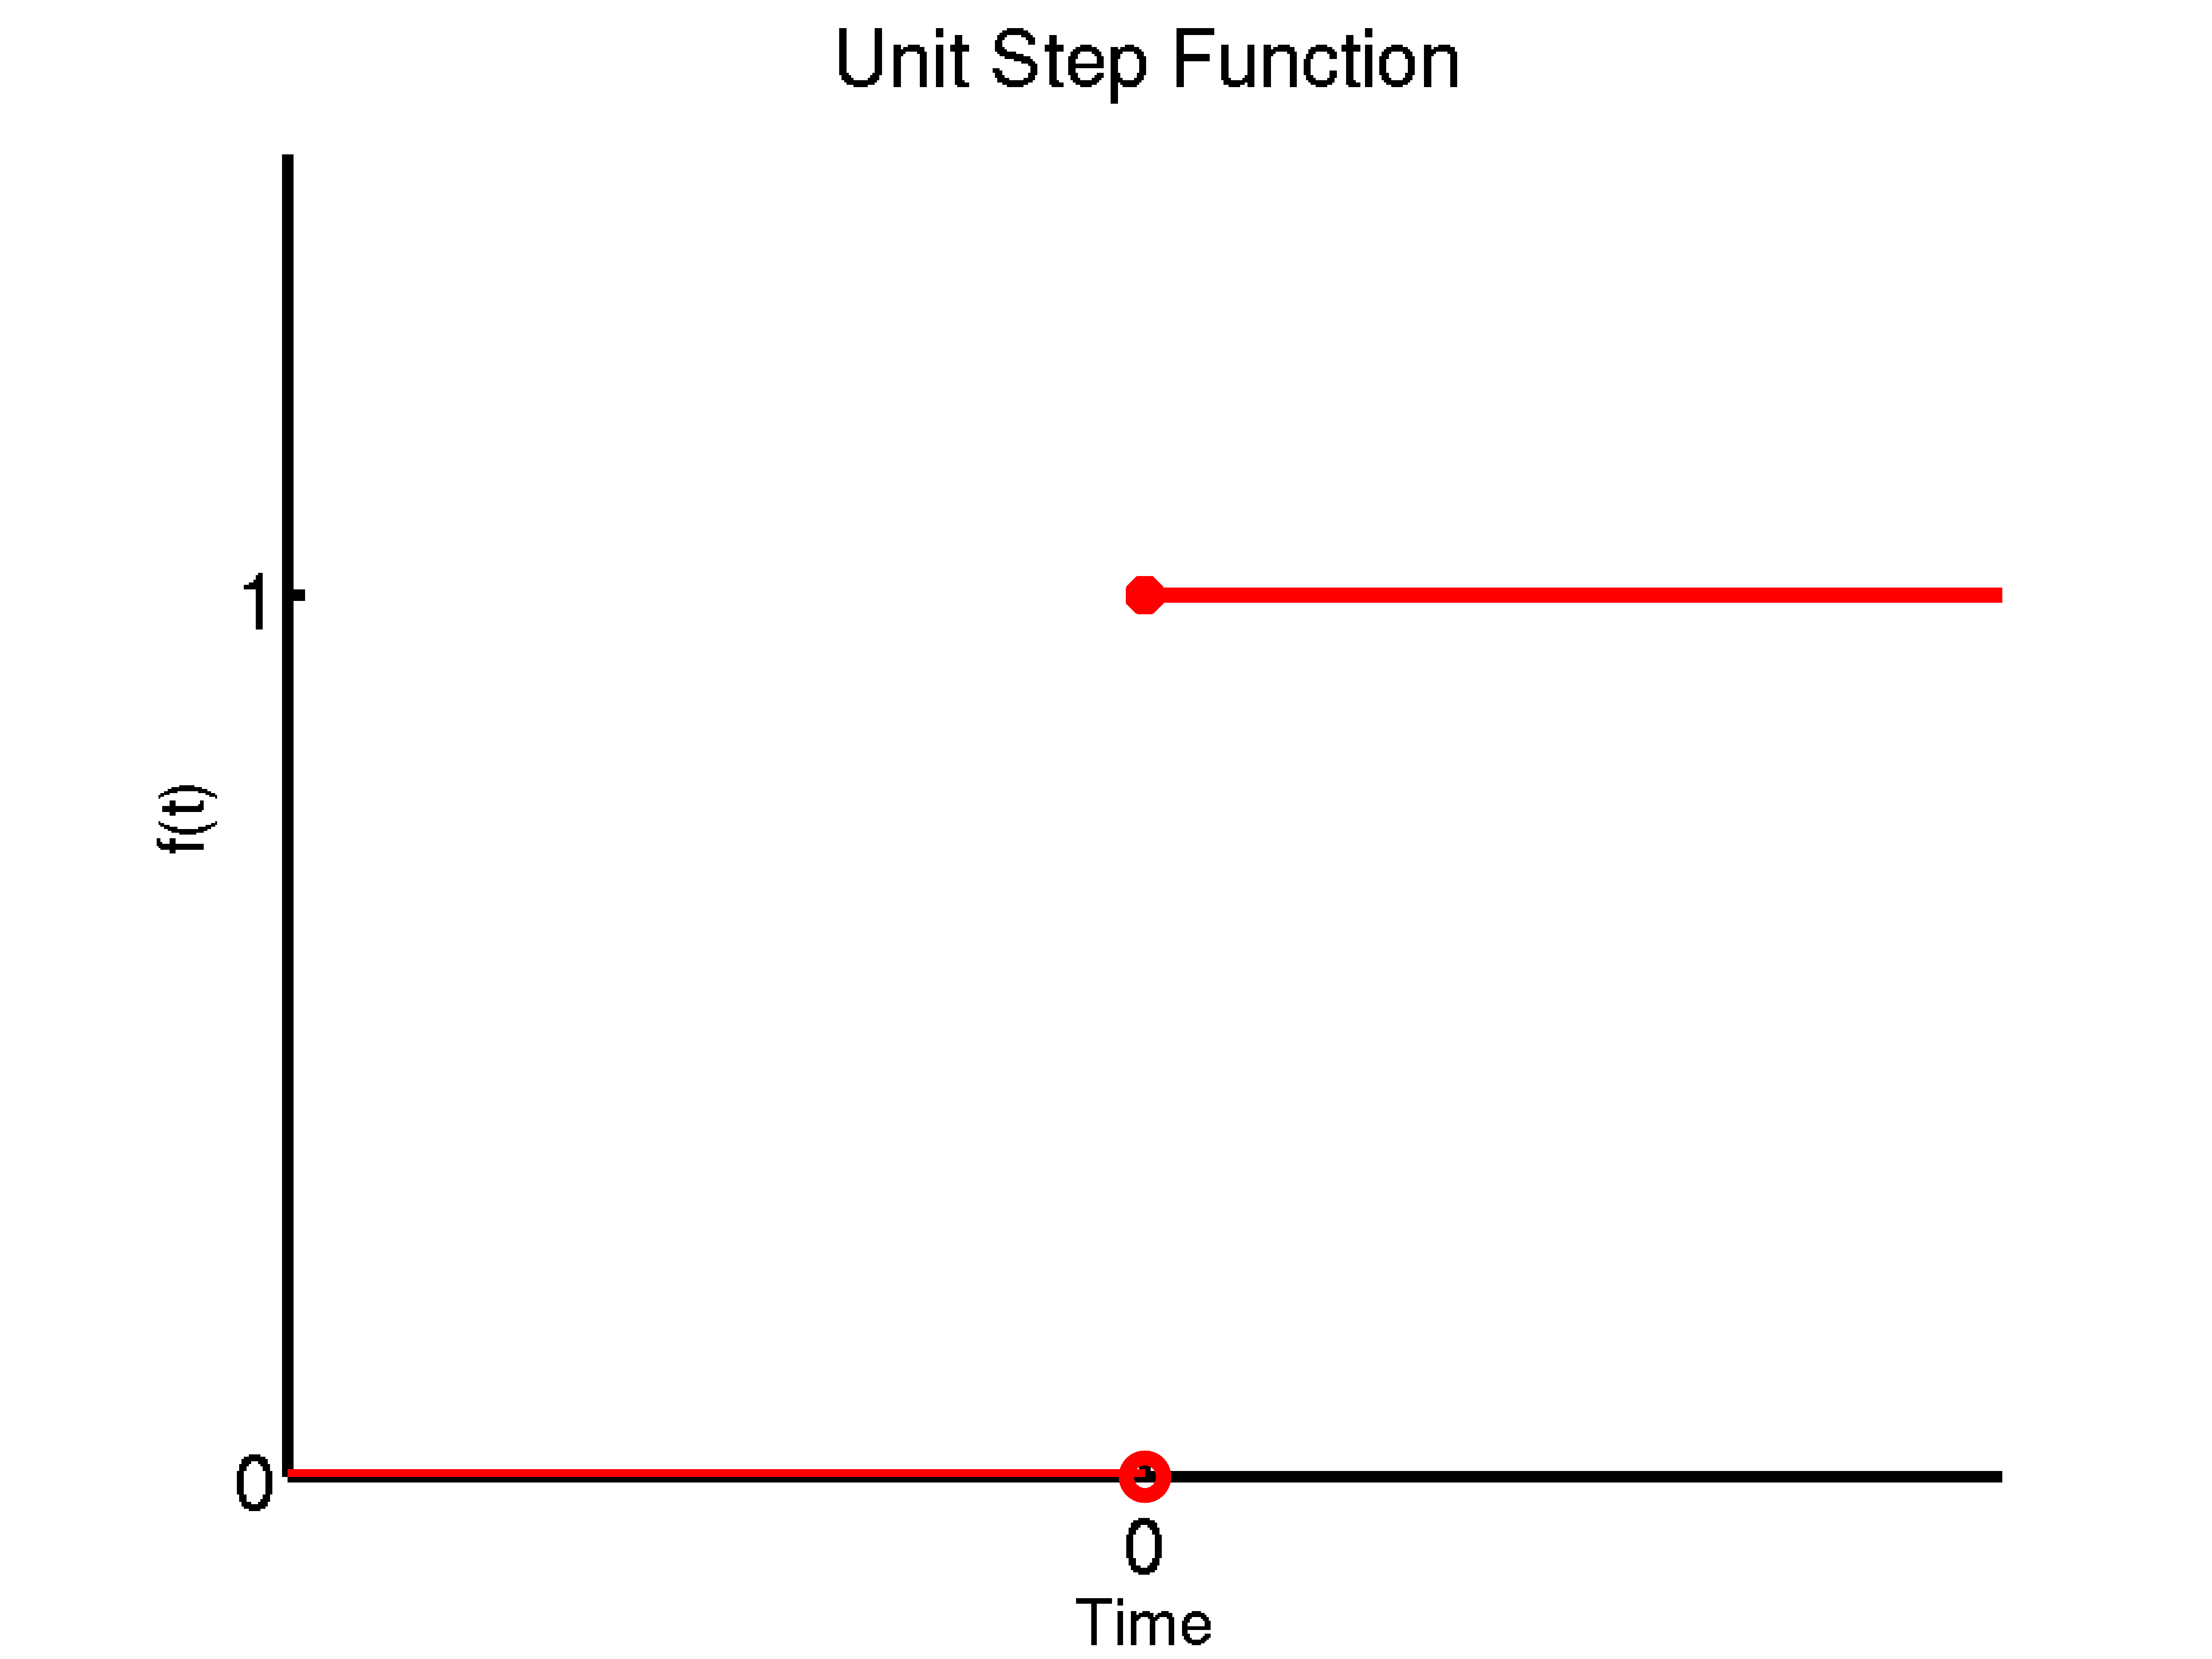
\includegraphics[width=5cm]{img/unitStepFunction}}

  A new name for an old function:
  \begin{eqnarray*}
    f(t) & = & 
    \left\{
      \begin{array}{r@{\hspace{2em}}rcl}
        1 & t & \geq & 0 \\
        0 & t & < & 0
      \end{array}
    \right.
  \end{eqnarray*}

  \uncover<2->
  {
    Define this to be
    \begin{eqnarray*}
      \mathrm{step}(t) & = & 
      \left\{
        \begin{array}{r@{\hspace{2em}}rcl}
          1 & t & \geq & 0 \\
          0 & t & < & 0
        \end{array}
      \right.
    \end{eqnarray*}
  }

\end{frame}


\begin{frame}
  \frametitle{Shifted Version}

  \centerline{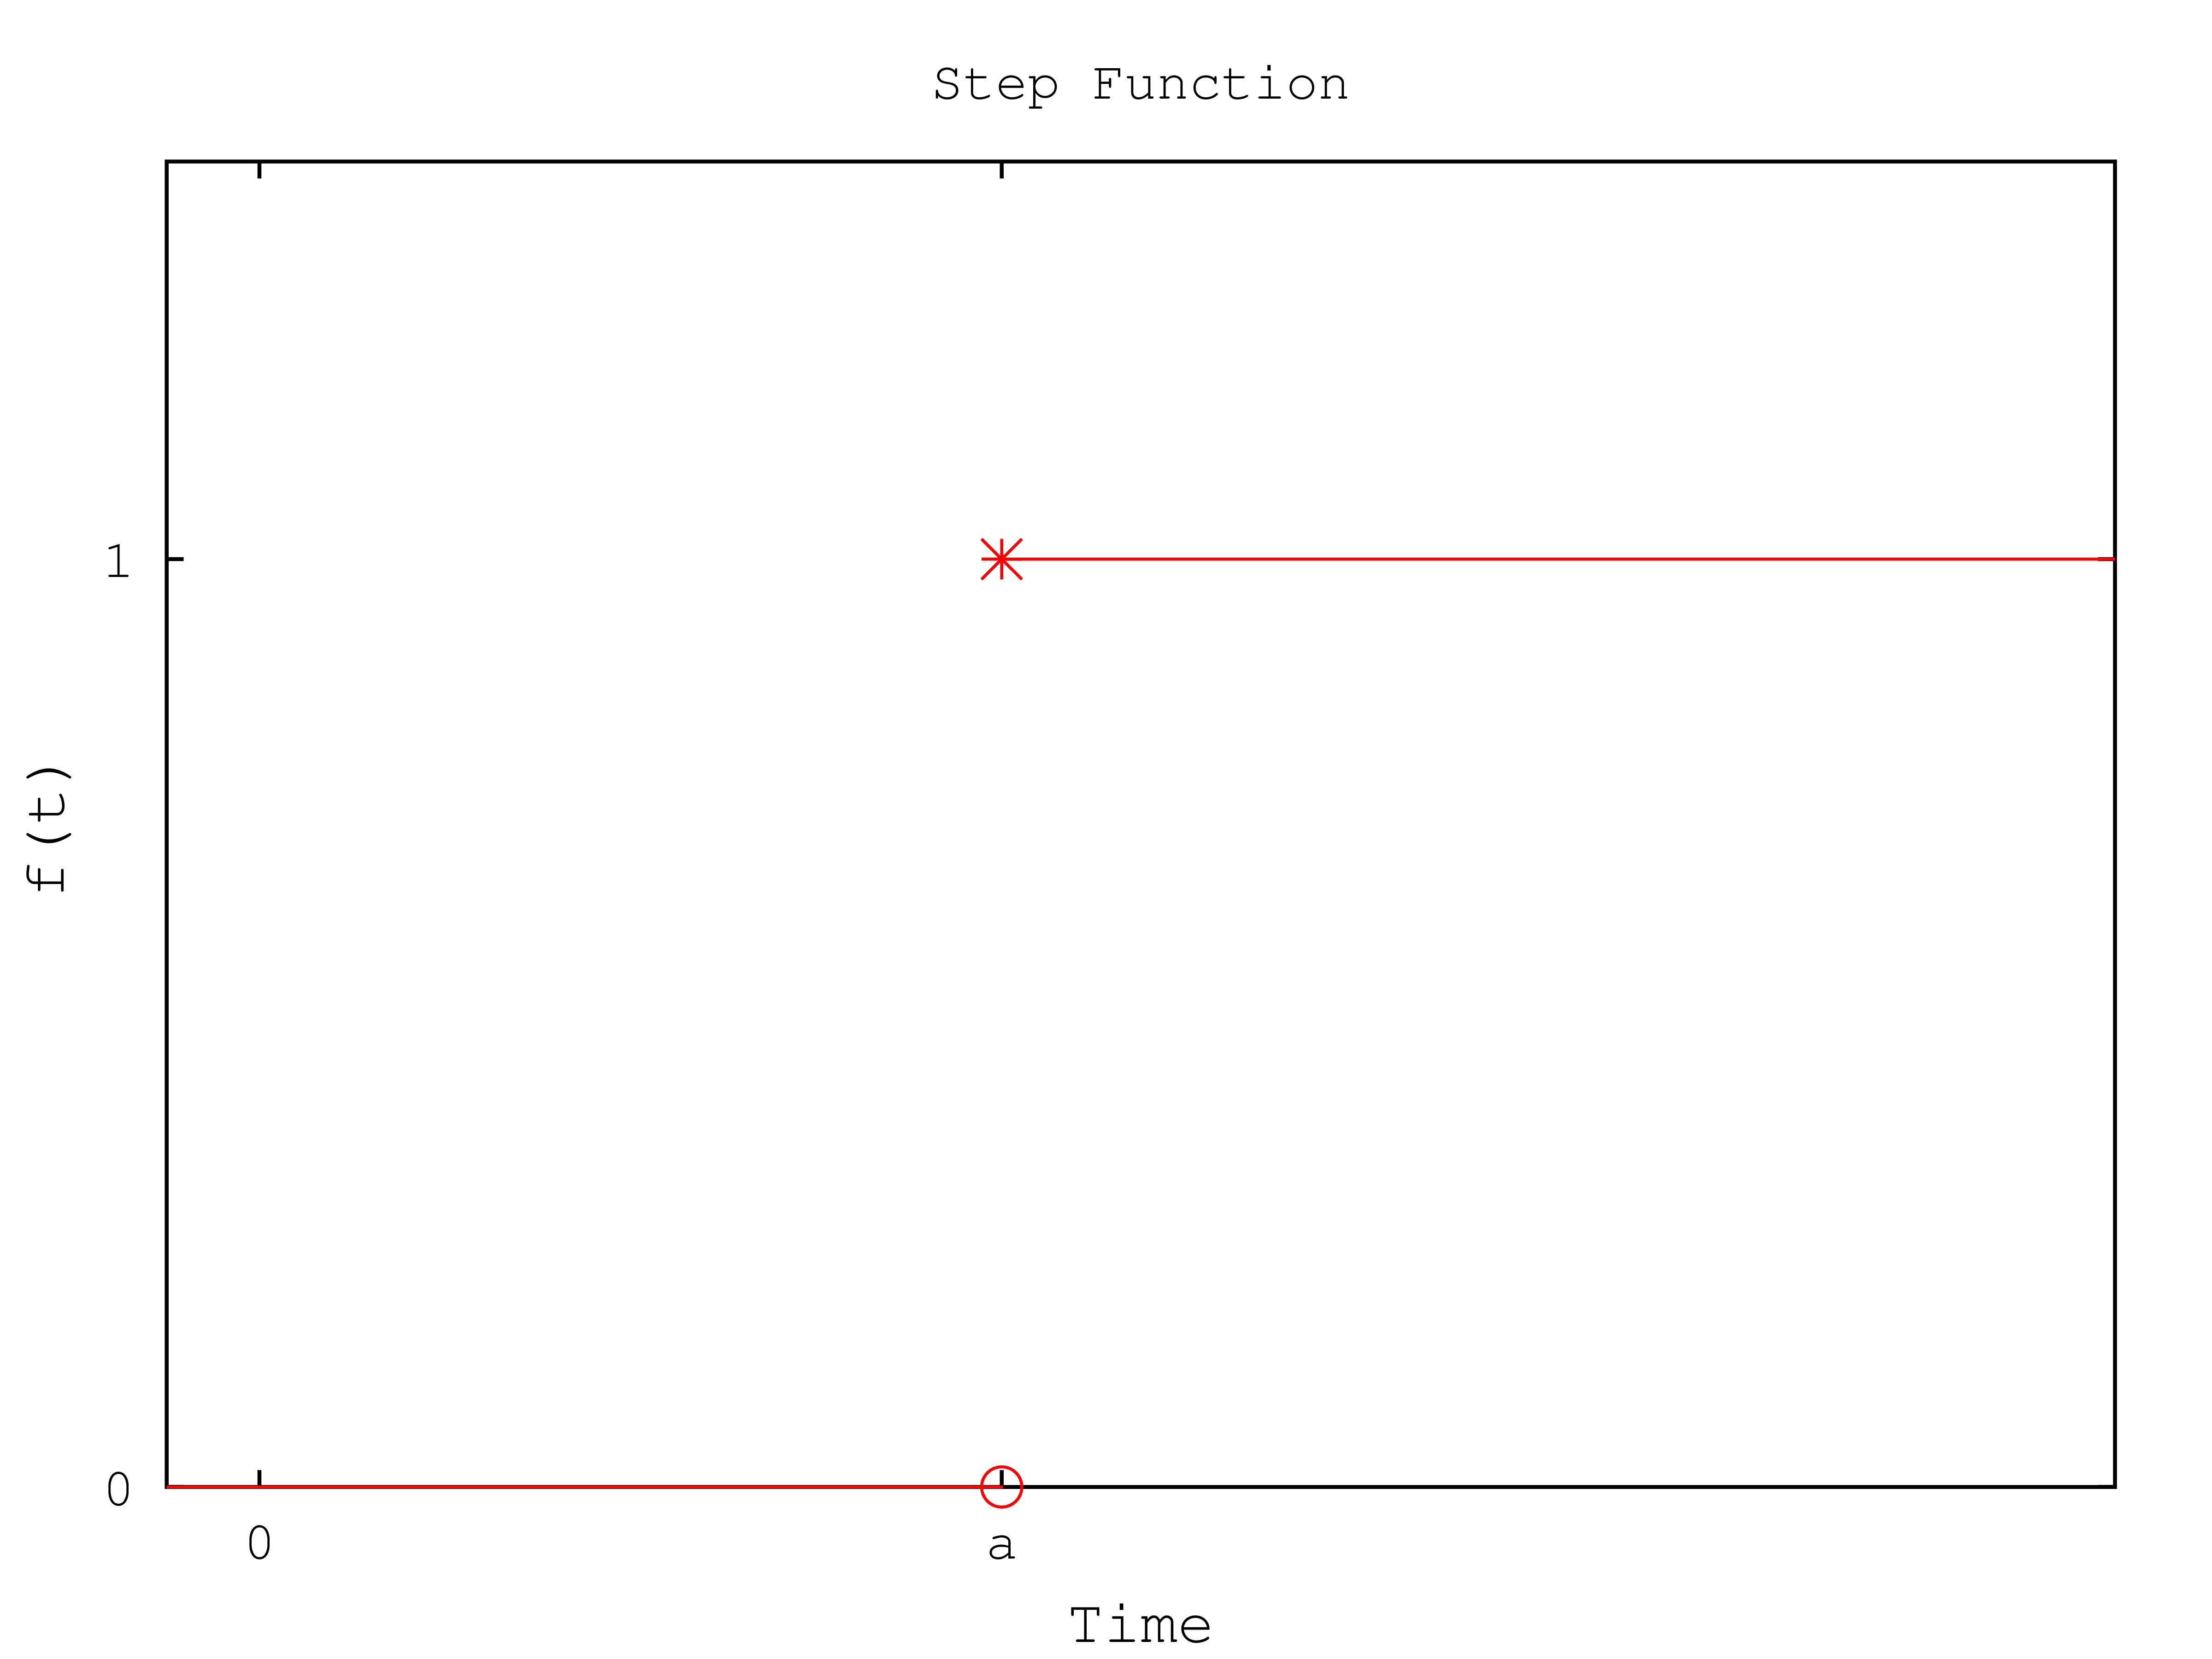
\includegraphics[width=5cm]{img/unitStepAta}}

    The function shifted $a$ units to the right is
    \begin{eqnarray*}
      \mathrm{step}(t-a) & = & 
      \left\{
        \begin{array}{r@{\hspace{2em}}rcl}
          1 & t & \geq & a \\
          0 & t & < & a
        \end{array}
      \right.
    \end{eqnarray*}


\end{frame}

\subsection{Examples Using the Unit Step Function}

\iftoggle{clicker}{%
\begin{frame}
  \frametitle{Clicker Quiz}

   \ifnum\value{clickerQuiz}=1{%
     Express the function
     \begin{eqnarray*}
       f(t) & = & 
       \left\{
         \begin{array}{r@{\hspace{2em}}rcl}
           2 & t & \geq & 0 \\
           0 & t & < & 0
         \end{array}
       \right.
     \end{eqnarray*}
     in terms of the unit step function.

     \vspace{2em}
     \begin{tabular}{ll}
       A: & step(t) \\ [12pt]
       B: & $2\cdot$step(t) \\ [12pt]
       C: & step(t-2)
     \end{tabular}

     \vfill
   }\fi

   \ifnum\value{clickerQuiz}=2{%
     Express the function
     \begin{eqnarray*}
       f(t) & = & 
       \left\{
         \begin{array}{r@{\hspace{2em}}rcl}
           2 & t & \geq & 0 \\
           0 & t & < & 0
         \end{array}
       \right.
     \end{eqnarray*}
     in terms of the unit step function.

     \vspace{2em}
     \begin{tabular}{ll}
       A: & step(t) \\ [12pt]
       B: & $2\cdot$step(t) \\ [12pt]
       C: & step(t-2)
     \end{tabular}

   \vfill
   }\fi

  \ifnum\value{clickerQuiz}=3{%
     Express the function
     \begin{eqnarray*}
       f(t) & = & 
       \left\{
         \begin{array}{r@{\hspace{2em}}rcl}
           5 & t & \geq & 0 \\
           0 & t & < & 0
         \end{array}
       \right.
     \end{eqnarray*}
     in terms of the unit step function.

     \vspace{2em}
     \begin{tabular}{ll}
       A: & step(t) \\ [12pt]
       B: & $5\cdot$step(t) \\ [12pt]
       C: & step(t-5)
     \end{tabular}

     \vfill
 }\fi
\end{frame}
}



\begin{frame}
  \frametitle{So What?}

  \centerline{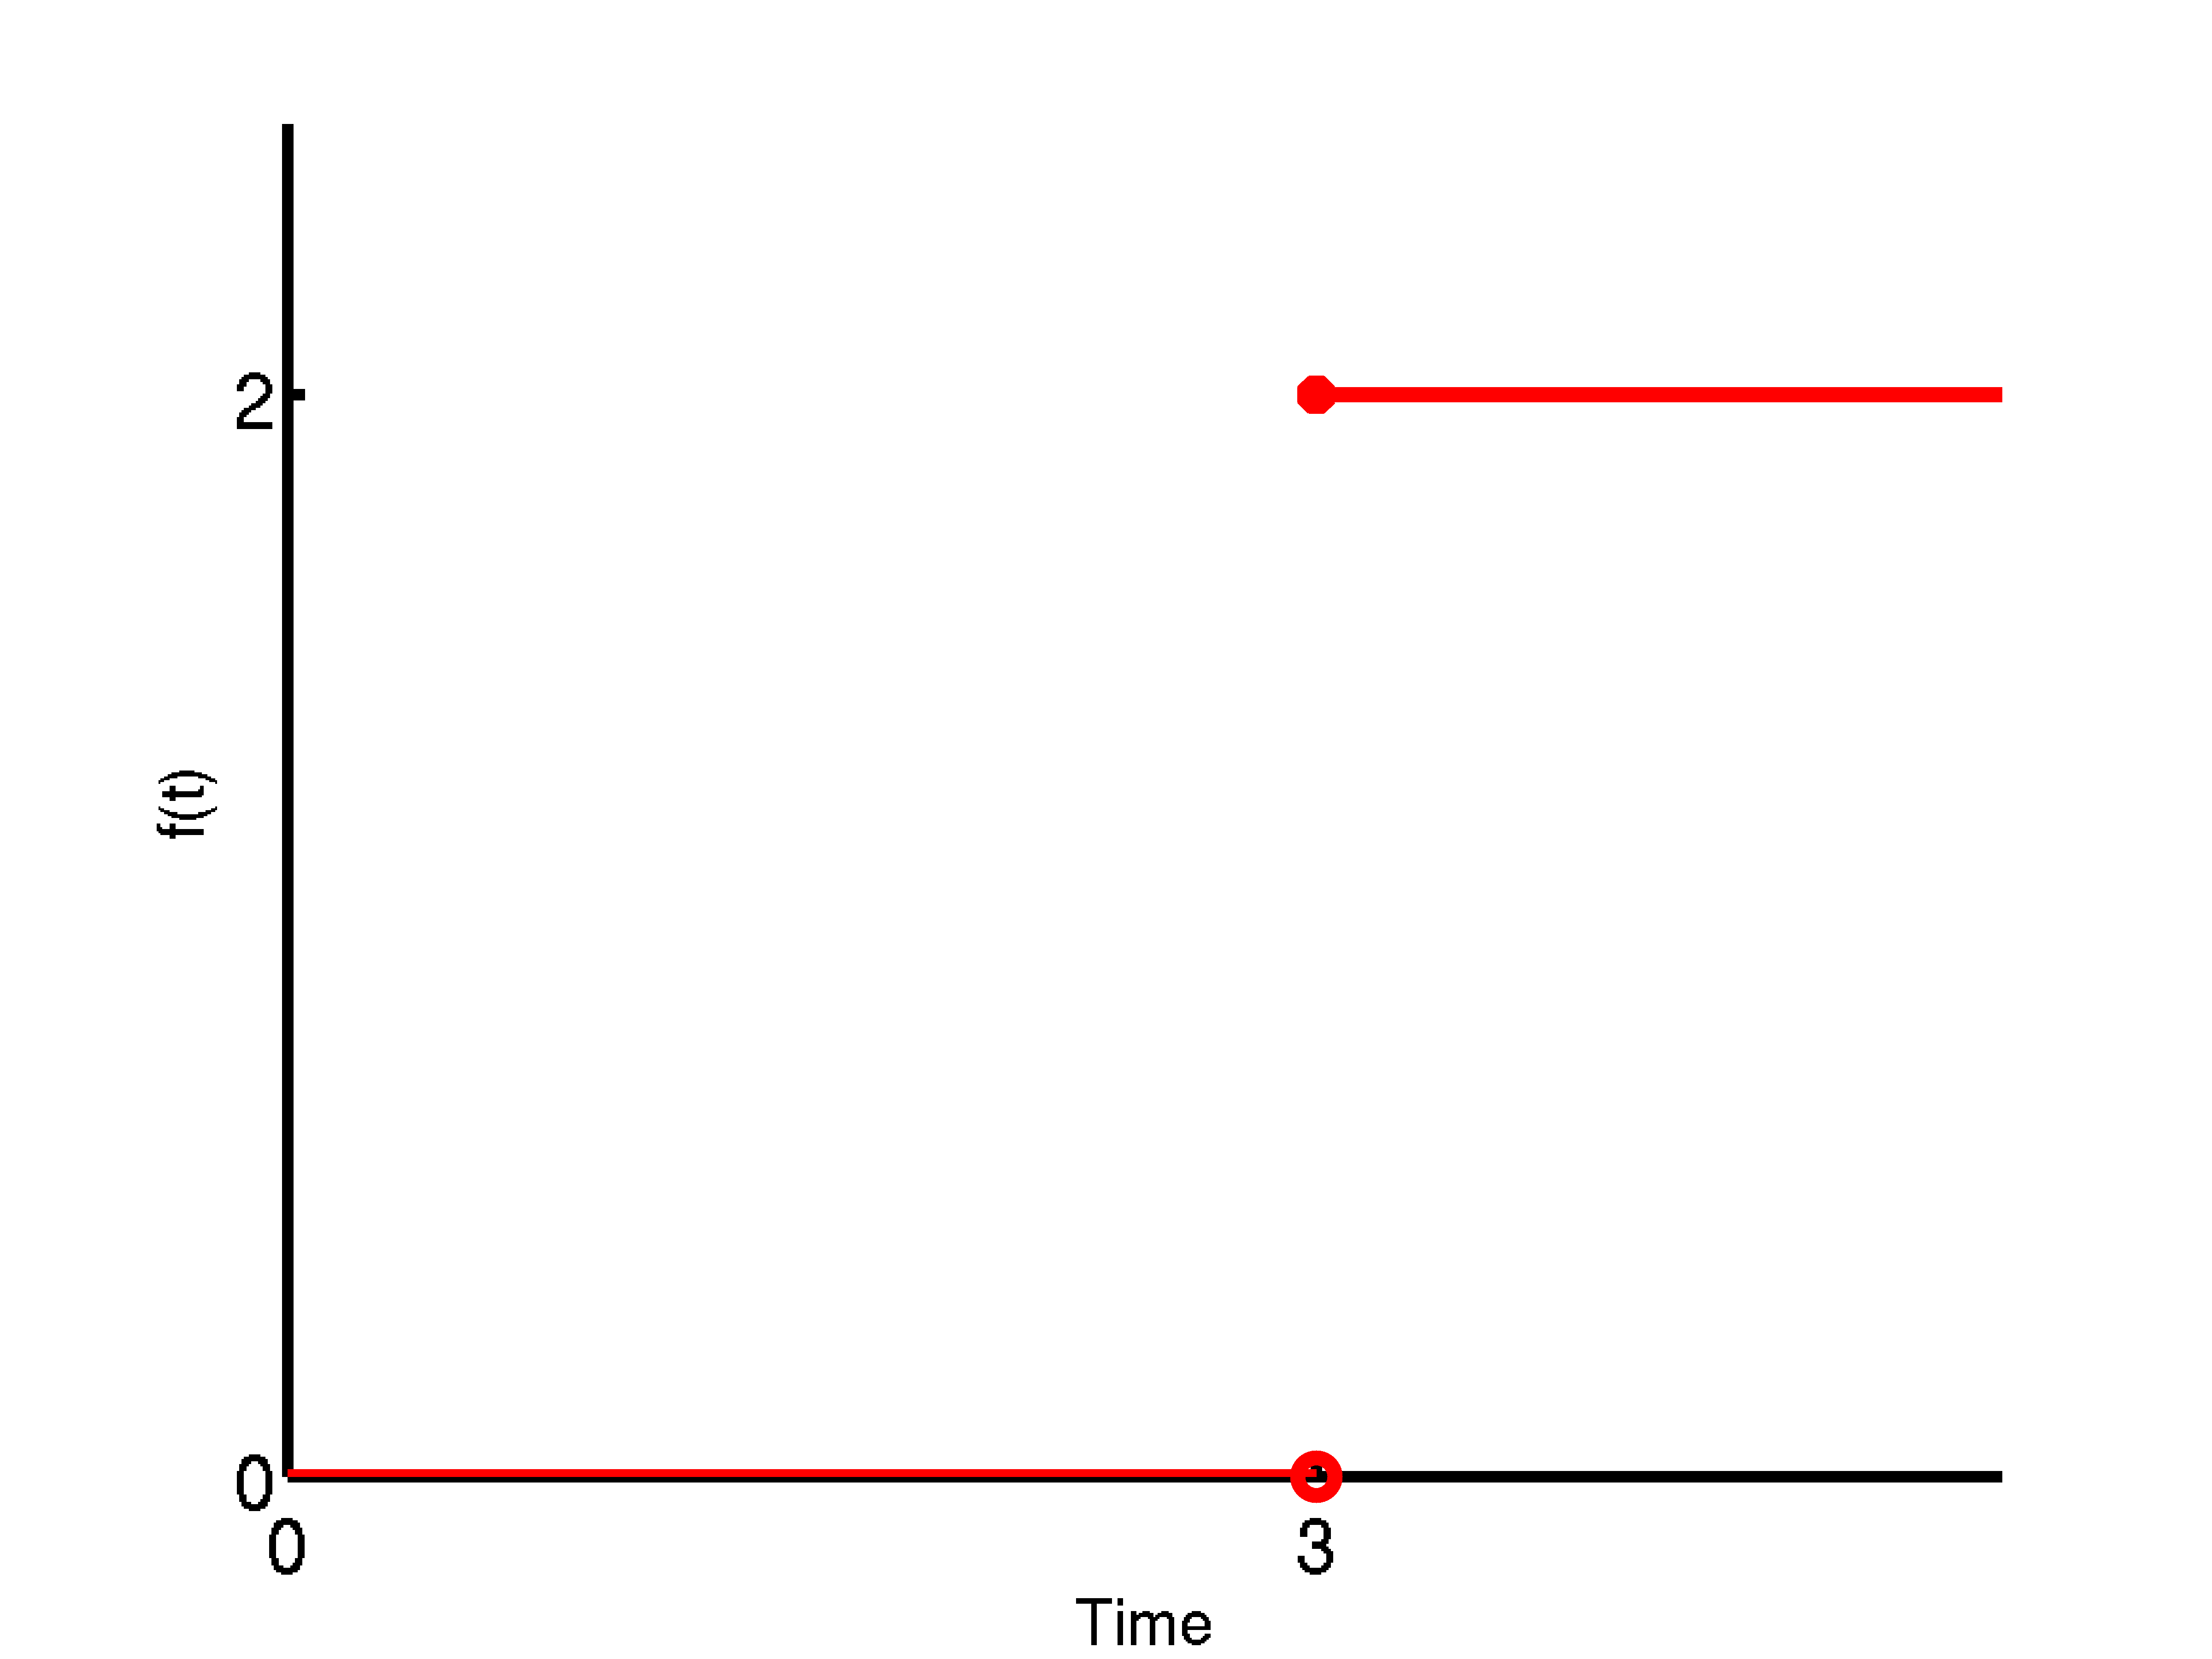
\includegraphics[width=5cm]{img/stepEx1}}

  \begin{eqnarray*}
      f(t) & = & 
      \left\{
        \begin{array}{r@{\hspace{2em}}rcl}
          2 & t & \geq & 3 \\
          0 & t & < & 3
        \end{array}
      \right.
  \end{eqnarray*}

  \uncover<2->
  {
    \begin{eqnarray*}
      f(t) & = & 2\mathrm{step}(t-3).
    \end{eqnarray*}
  }

\end{frame}


\iftoggle{clicker}{%
\begin{frame}
  \frametitle{Clicker Quiz}

   \ifnum\value{clickerQuiz}=1{%
     Express the function
     \begin{eqnarray*}
       f(t) & = & 
       \left\{
         \begin{array}{r@{\hspace{2em}}rcl}
           0 & t & \geq & 0 \\
           1 & t & < & 0
         \end{array}
       \right.
     \end{eqnarray*}
     in terms of the unit step function.

     \vspace{2em}
     \begin{tabular}{ll}
       A: & -step(t) \\ [12pt]
       B: & $1-$step(t) \\ [12pt]
       C: & step(t-1)
     \end{tabular}

     \vfill
   }\fi

   \ifnum\value{clickerQuiz}=2{%
     Express the function
     \begin{eqnarray*}
       f(t) & = & 
       \left\{
         \begin{array}{r@{\hspace{2em}}rcl}
           0 & t & \geq & 0 \\
           1 & t & < & 0
         \end{array}
       \right.
     \end{eqnarray*}
     in terms of the unit step function.

     \vspace{2em}
     \begin{tabular}{ll}
       A: & -step(t) \\ [12pt]
       B: & $1-$step(t) \\ [12pt]
       C: & step(t-1)
     \end{tabular}

   \vfill
   }\fi

  \ifnum\value{clickerQuiz}=3{%

     Express the function
     \begin{eqnarray*}
       f(t) & = & 
       \left\{
         \begin{array}{r@{\hspace{2em}}rcl}
           0 & t & \geq & 0 \\
           1 & t & < & 0
         \end{array}
       \right.
     \end{eqnarray*}
     in terms of the unit step function.

     \vspace{2em}
     \begin{tabular}{ll}
       A: & -step(t) \\ [12pt]
       B: & $1-$step(t) \\ [12pt]
       C: & step(t-1)
     \end{tabular}

    \vfill
 }\fi
\end{frame}
}


\begin{frame}
  \frametitle{A little bit harder now}

  \centerline{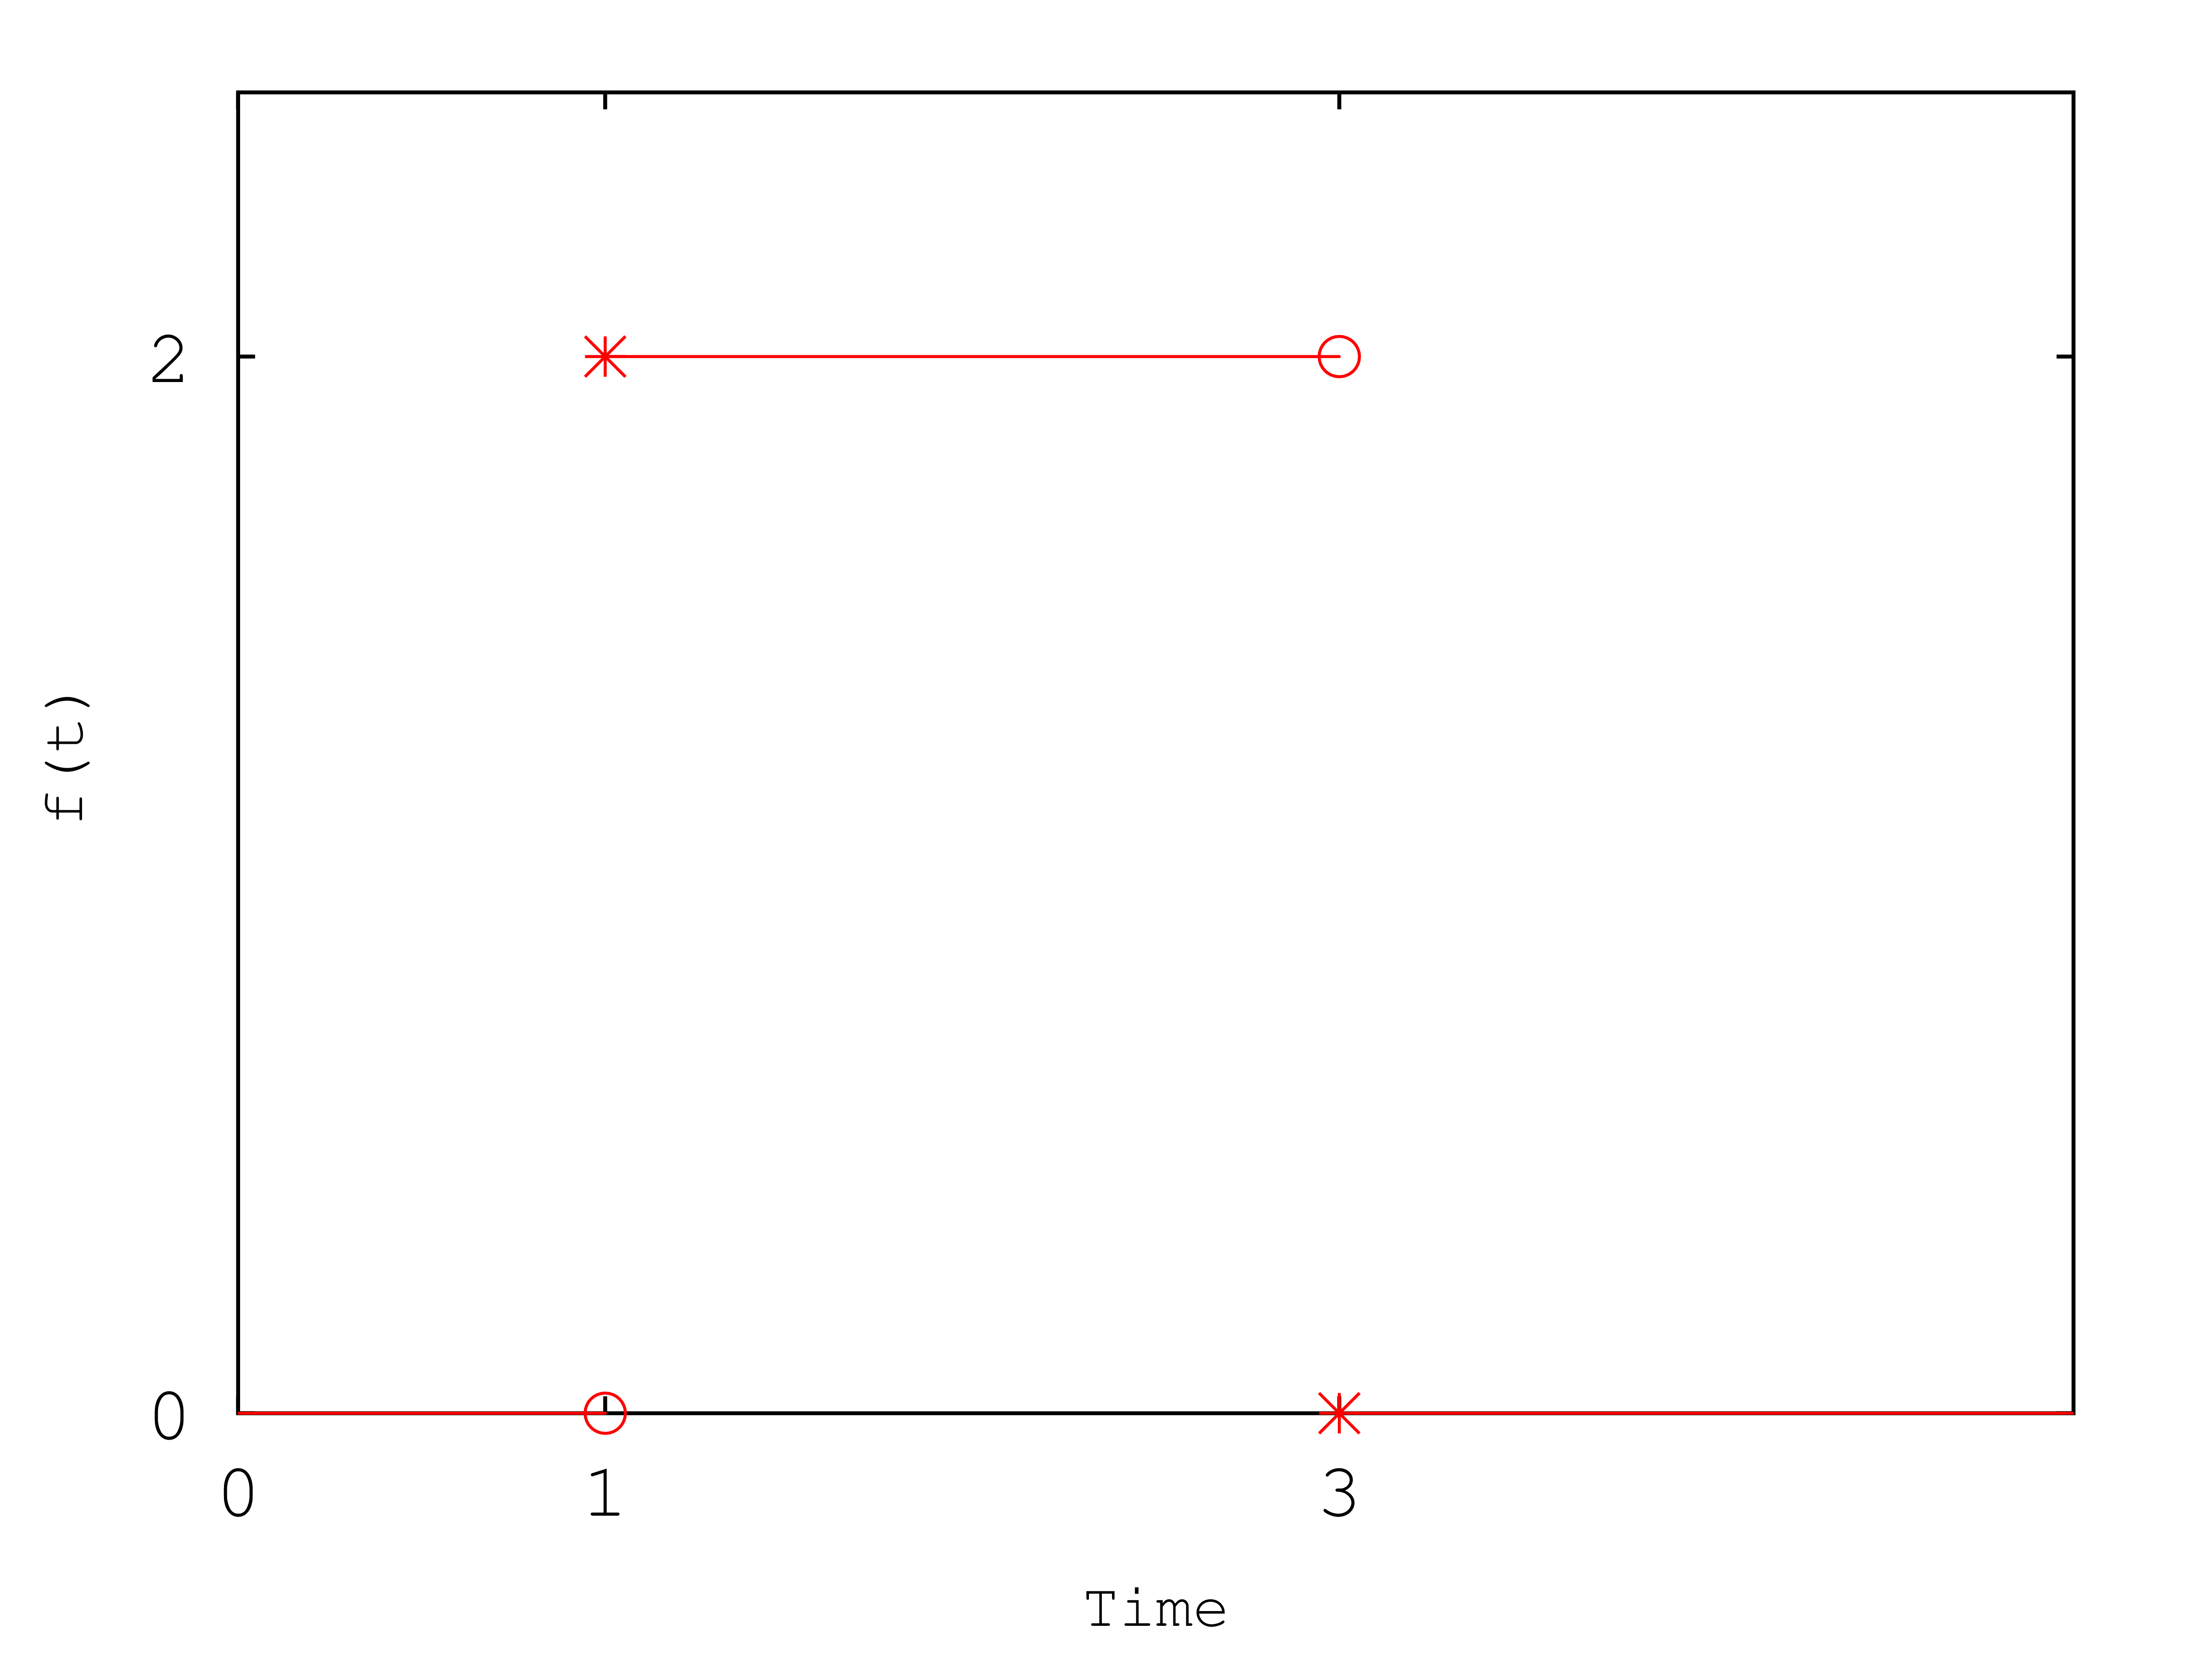
\includegraphics[width=5cm]{img/stepEx2}}

  \begin{eqnarray*}
      f(t) & = & 
      \left\{
        \begin{array}{rr}
          2 & 1\leq t < 3 \\
          0 & \mathrm{otherwise}
        \end{array}
      \right.
  \end{eqnarray*}

  \uncover<2->
  {
    \begin{eqnarray*}
      f(t) & = & 2\cdot\mathrm{step}(t-1) - 2\cdot\mathrm{step}(t-3).
    \end{eqnarray*}
  }

\end{frame}

\begin{frame}
  \frametitle{A little bit harder now}

  \centerline{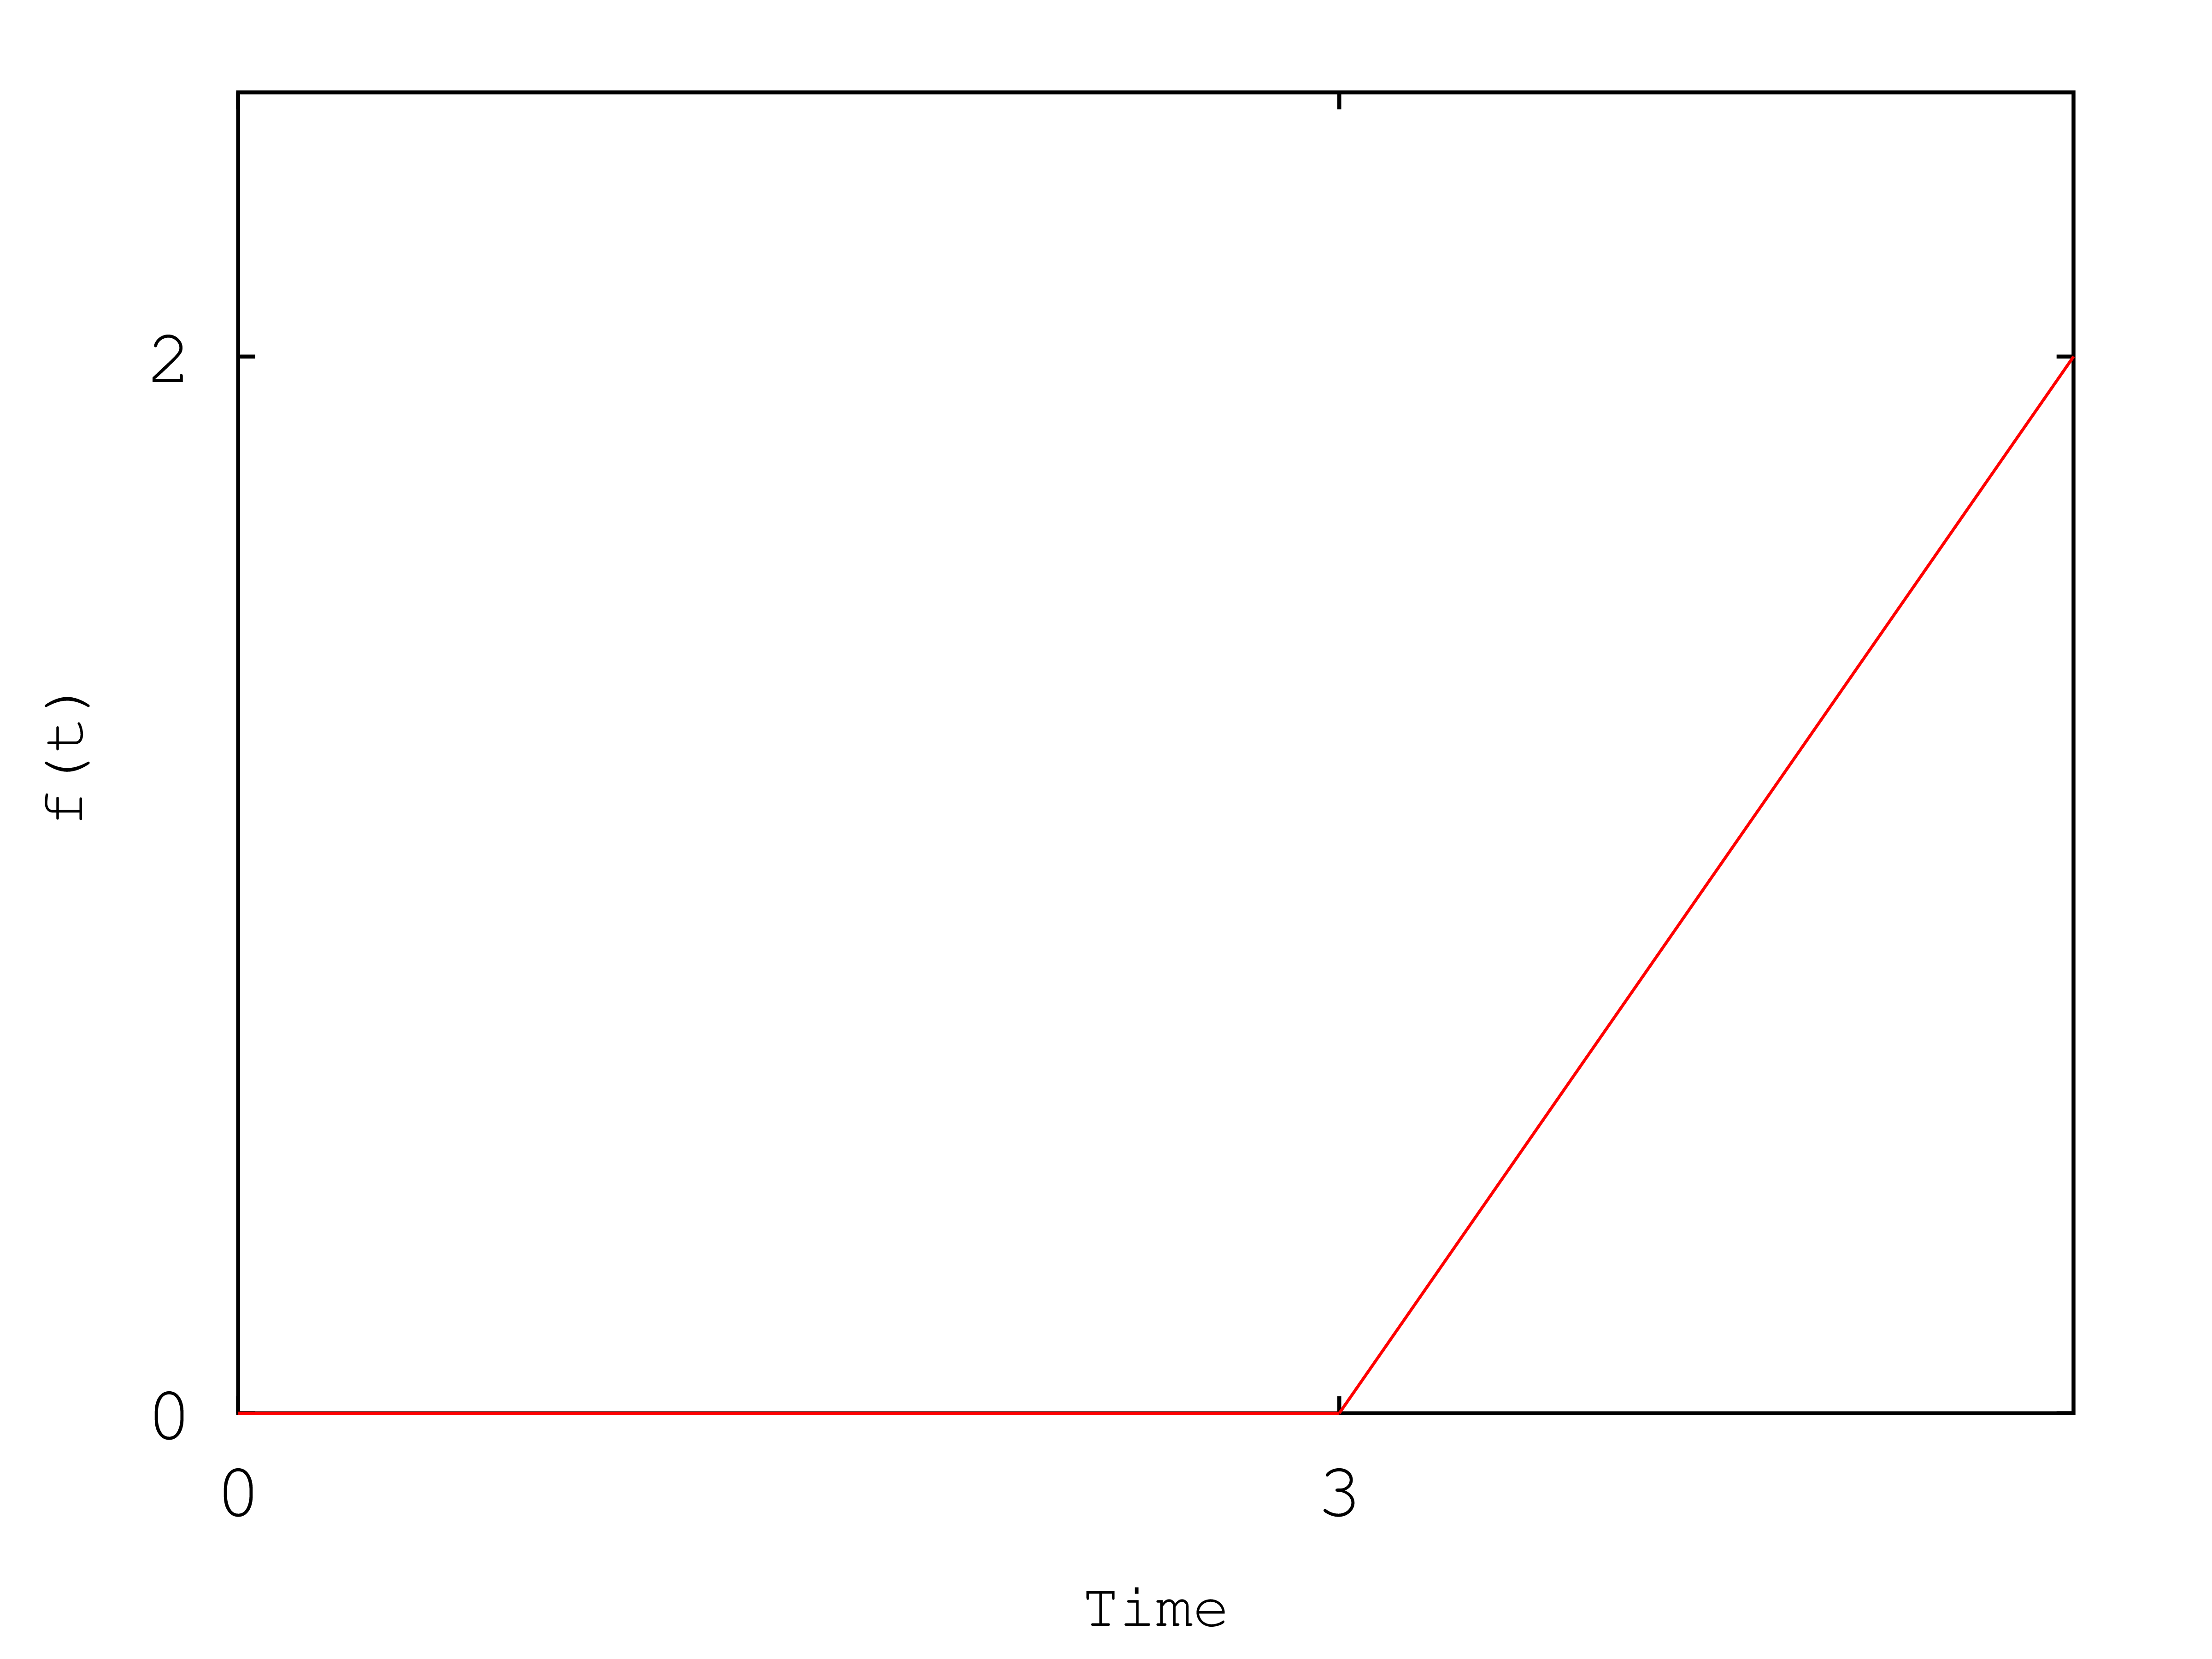
\includegraphics[width=5cm]{img/stepEx3}}

  \begin{eqnarray*}
      f(t) & = & 
      \left\{
        \begin{array}{rr}
          t-2 & 1\leq t < 3 \\
          0 & \mathrm{otherwise}
        \end{array}
      \right.
  \end{eqnarray*}

  \uncover<2->
  {
    \begin{eqnarray*}
      f(t) & = & (t-2)\cdot\mathrm{step}(t-1) - (t-2)\cdot\mathrm{step}(t-3).
    \end{eqnarray*}
  }

\end{frame}

\begin{frame}
  \frametitle{A little bit harder now}

  \centerline{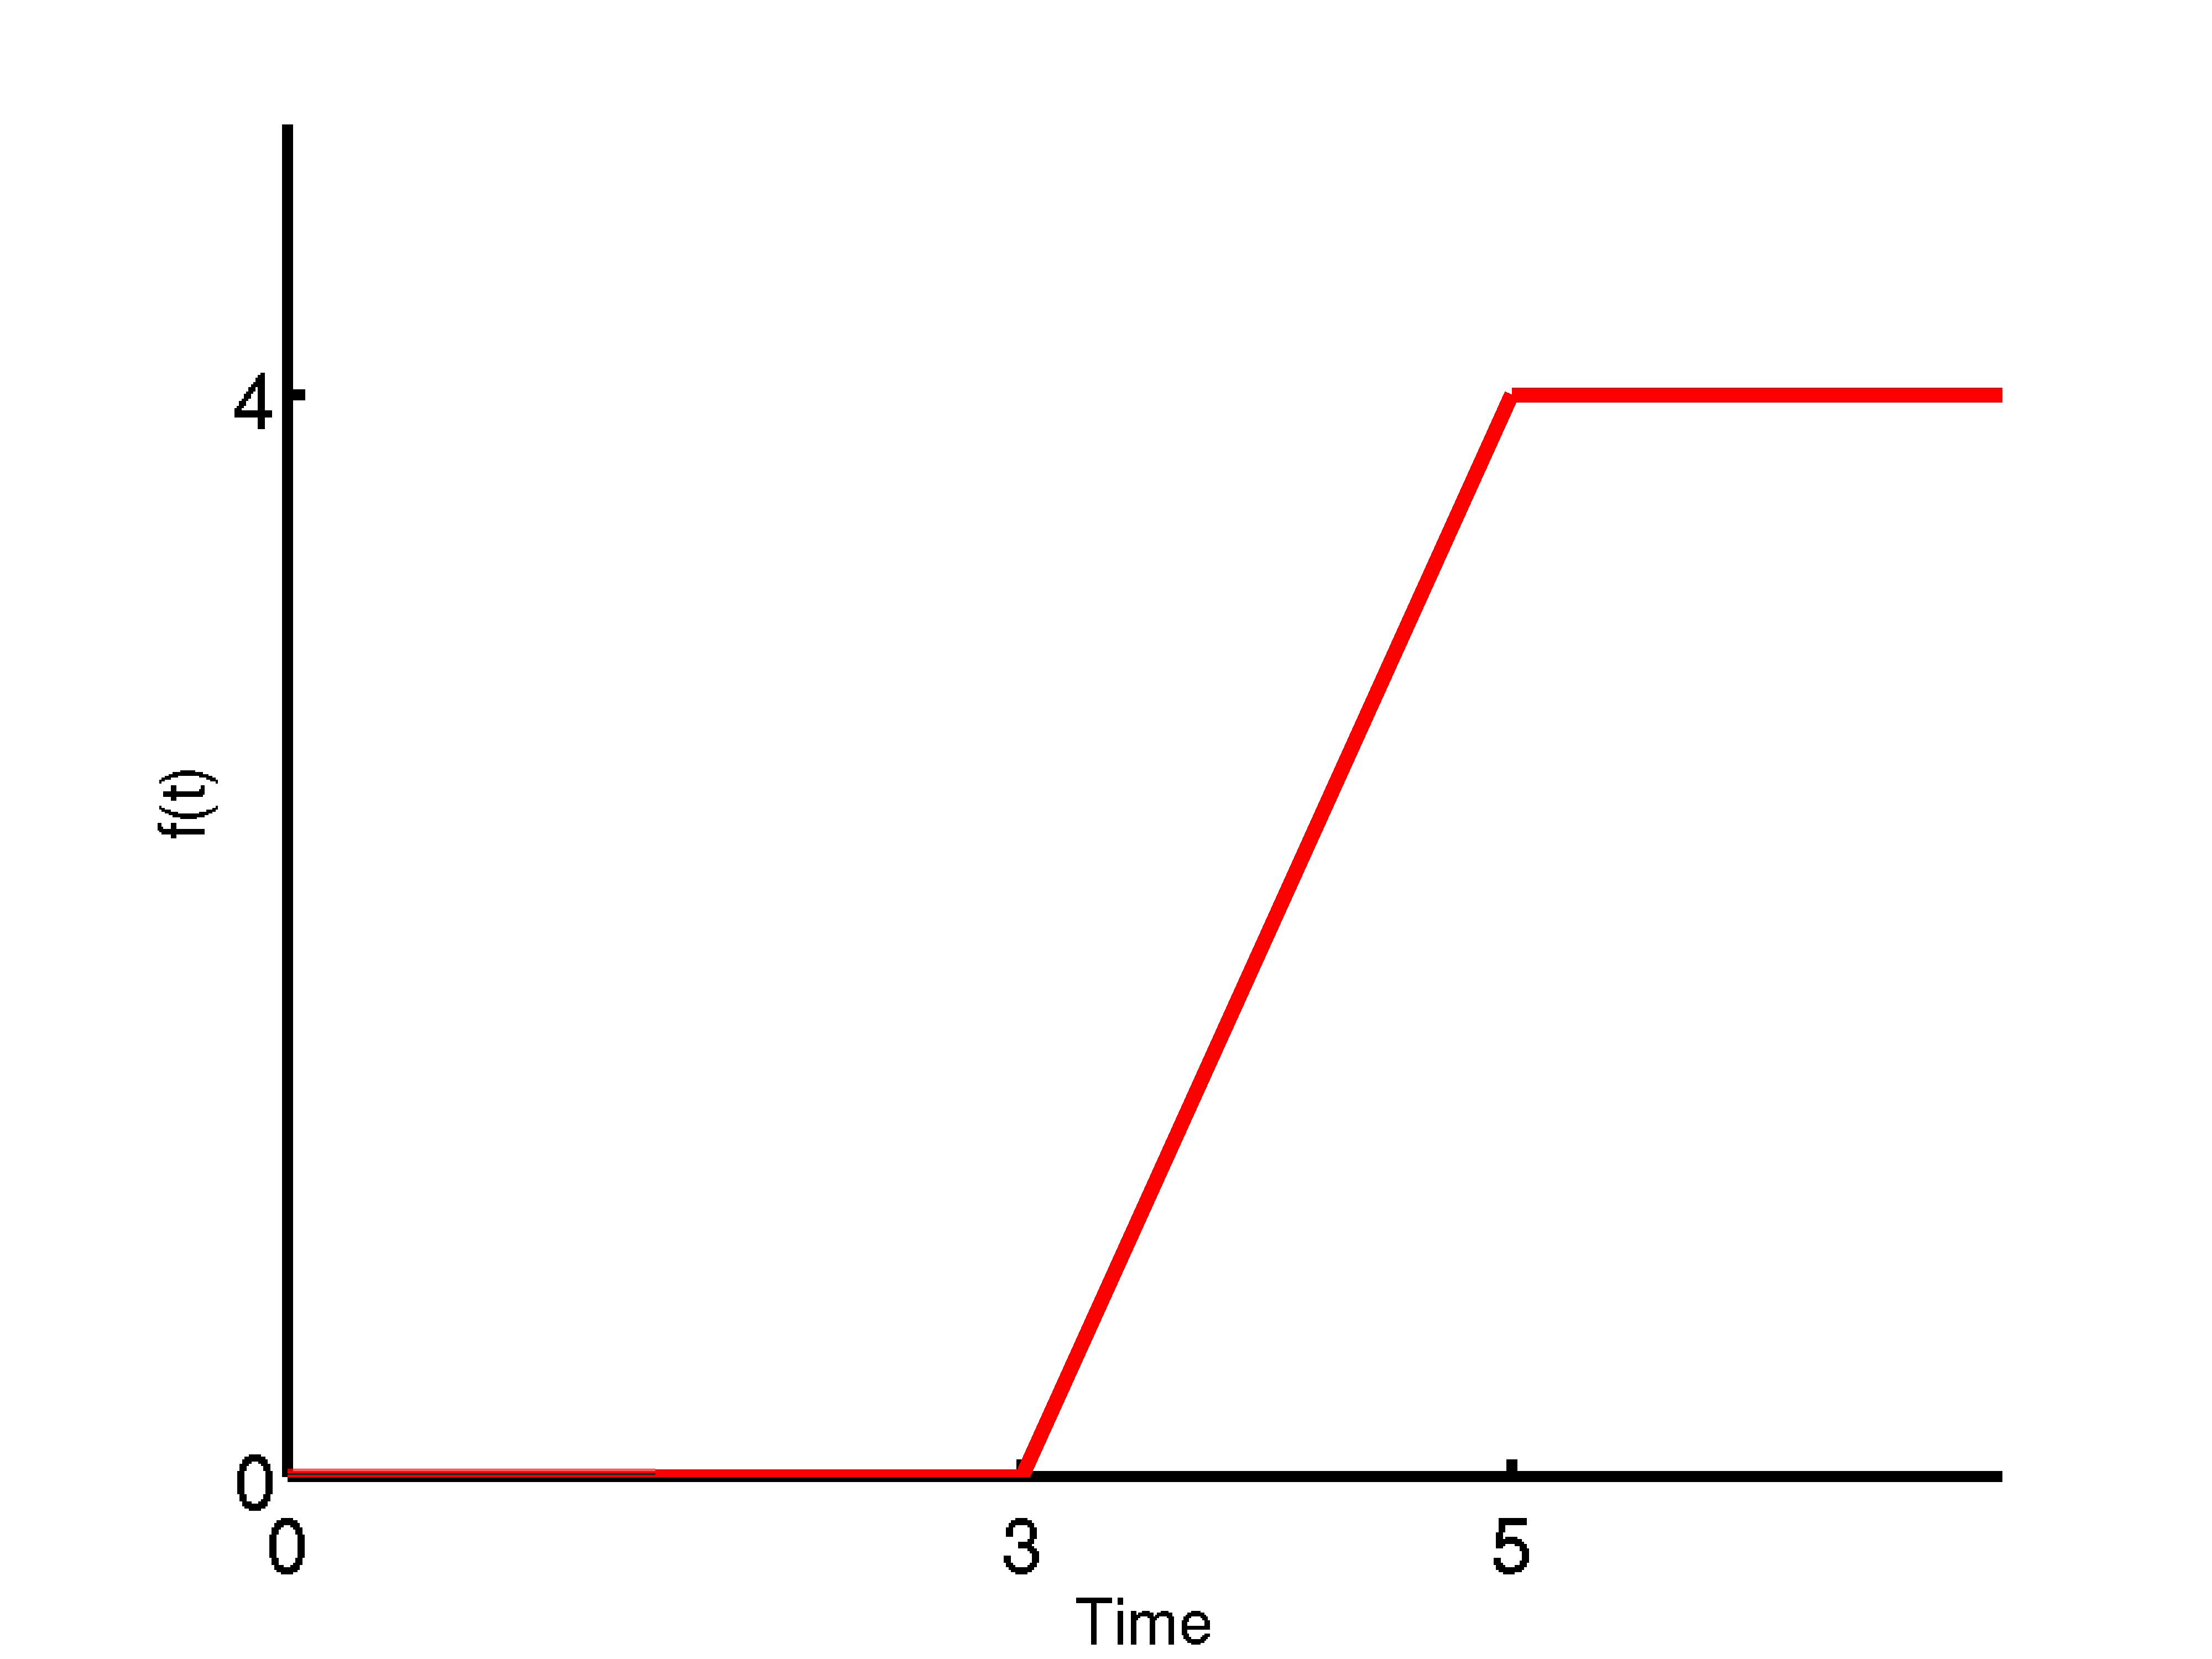
\includegraphics[width=5cm]{img/stepEx4}}

  \begin{eqnarray*}
      f(t) & = & 
      \left\{
        \begin{array}{r@{\hspace{2em}}rcccl}
          4 & t & \geq & 5 \\
          2(t-3) & 3 & < & t & < & 5 \\
          0 & t & \leq 3 
        \end{array}
      \right.
  \end{eqnarray*}

  \uncover<2->
  {
    \begin{eqnarray*}
      f(t) & = & 2(t-3)\cdot\mathrm{step}(t-3) -
                 2(t-3)\cdot\mathrm{step}(t-5) + \\
           &   & 4\cdot\mathrm{step}(t-5).
    \end{eqnarray*}
  }


\end{frame}


\begin{frame}
  \frametitle{A little bit harder now}

  \centerline{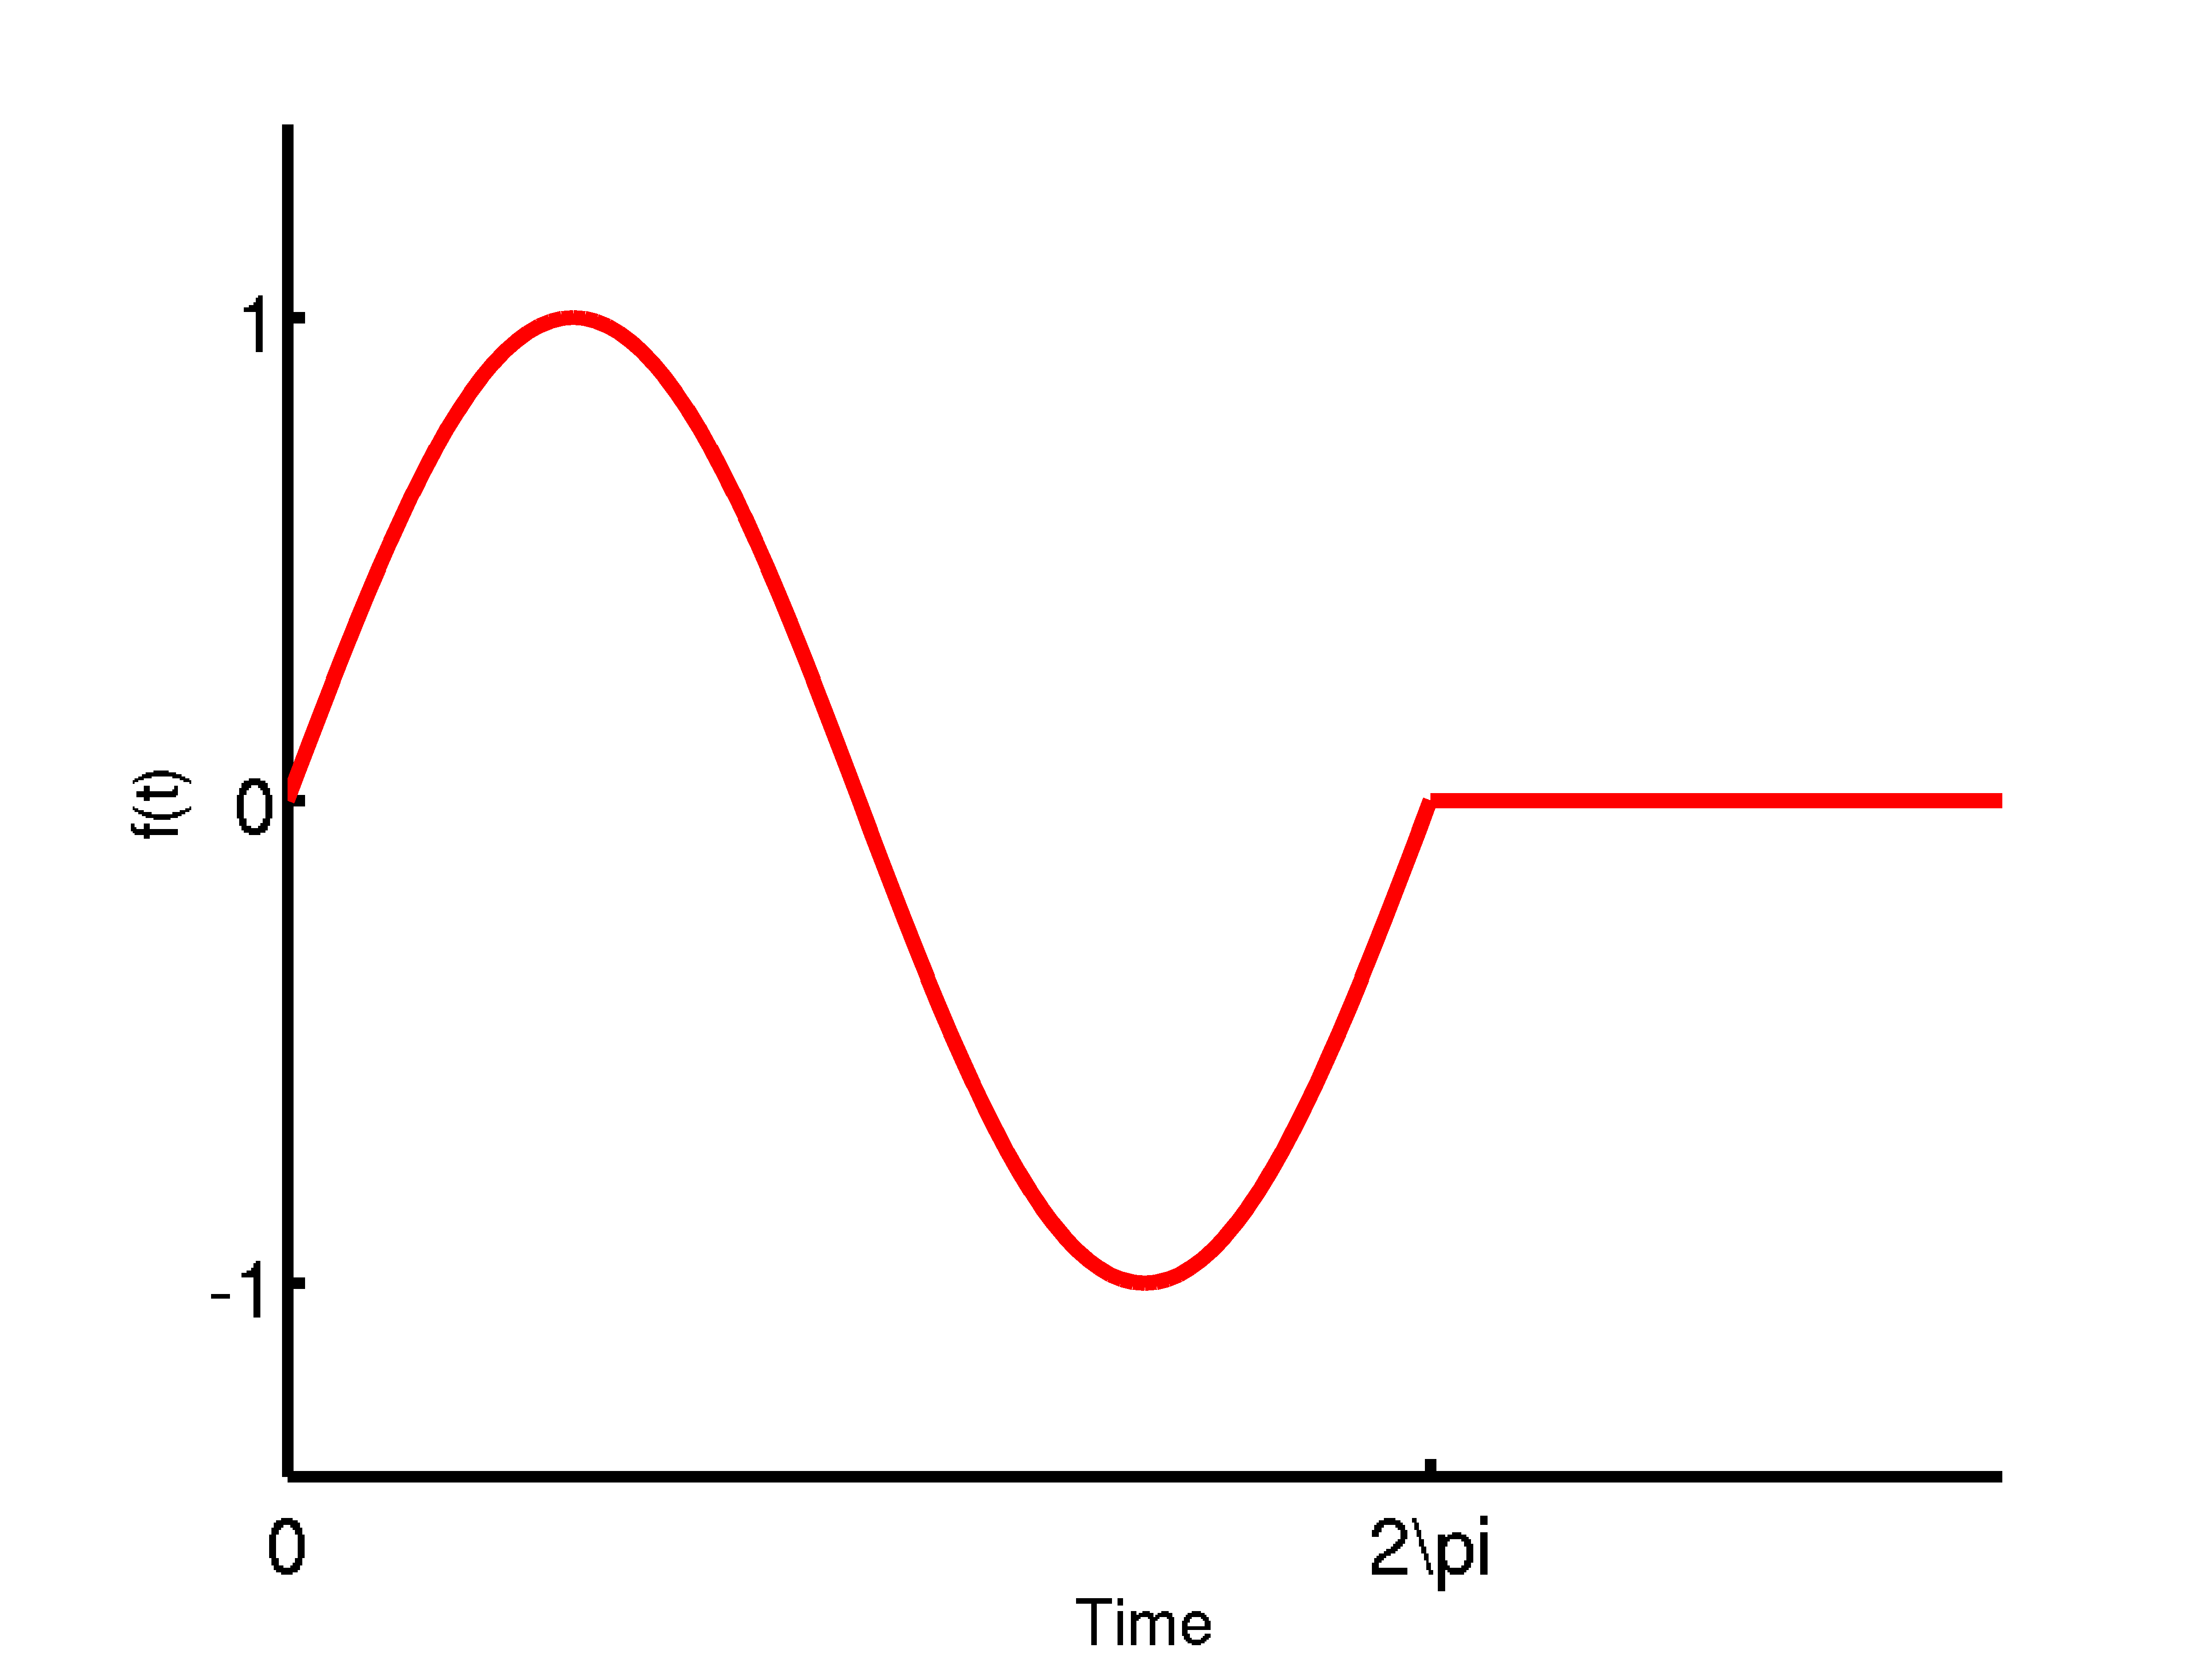
\includegraphics[width=4cm]{img/stepEx5}}

  \begin{eqnarray*}
      f(t) & = & 
      \left\{
        \begin{array}{r@{\hspace{2em}}r}
          \sin(t) & 0 \leq t \leq 2\pi \\
          0 &  \mathrm{otherwise}.
        \end{array}
      \right.
  \end{eqnarray*}

  \uncover<2->
  {
    \begin{eqnarray*}
      f(t) & = & \sin(t)\mathrm{step}(t-0) - \sin(t)\mathrm{step}(t-2\pi).
    \end{eqnarray*}
  }


  \uncover<3->
  {
    If we assume that $t\geq 0$:
    \begin{eqnarray*}
      f(t) & = & \sin(t) - \sin(t)\mathrm{step}(t-2\pi).
    \end{eqnarray*}
  }


\end{frame}



\begin{frame}
  \frametitle{A little bit harder now}

  \centerline{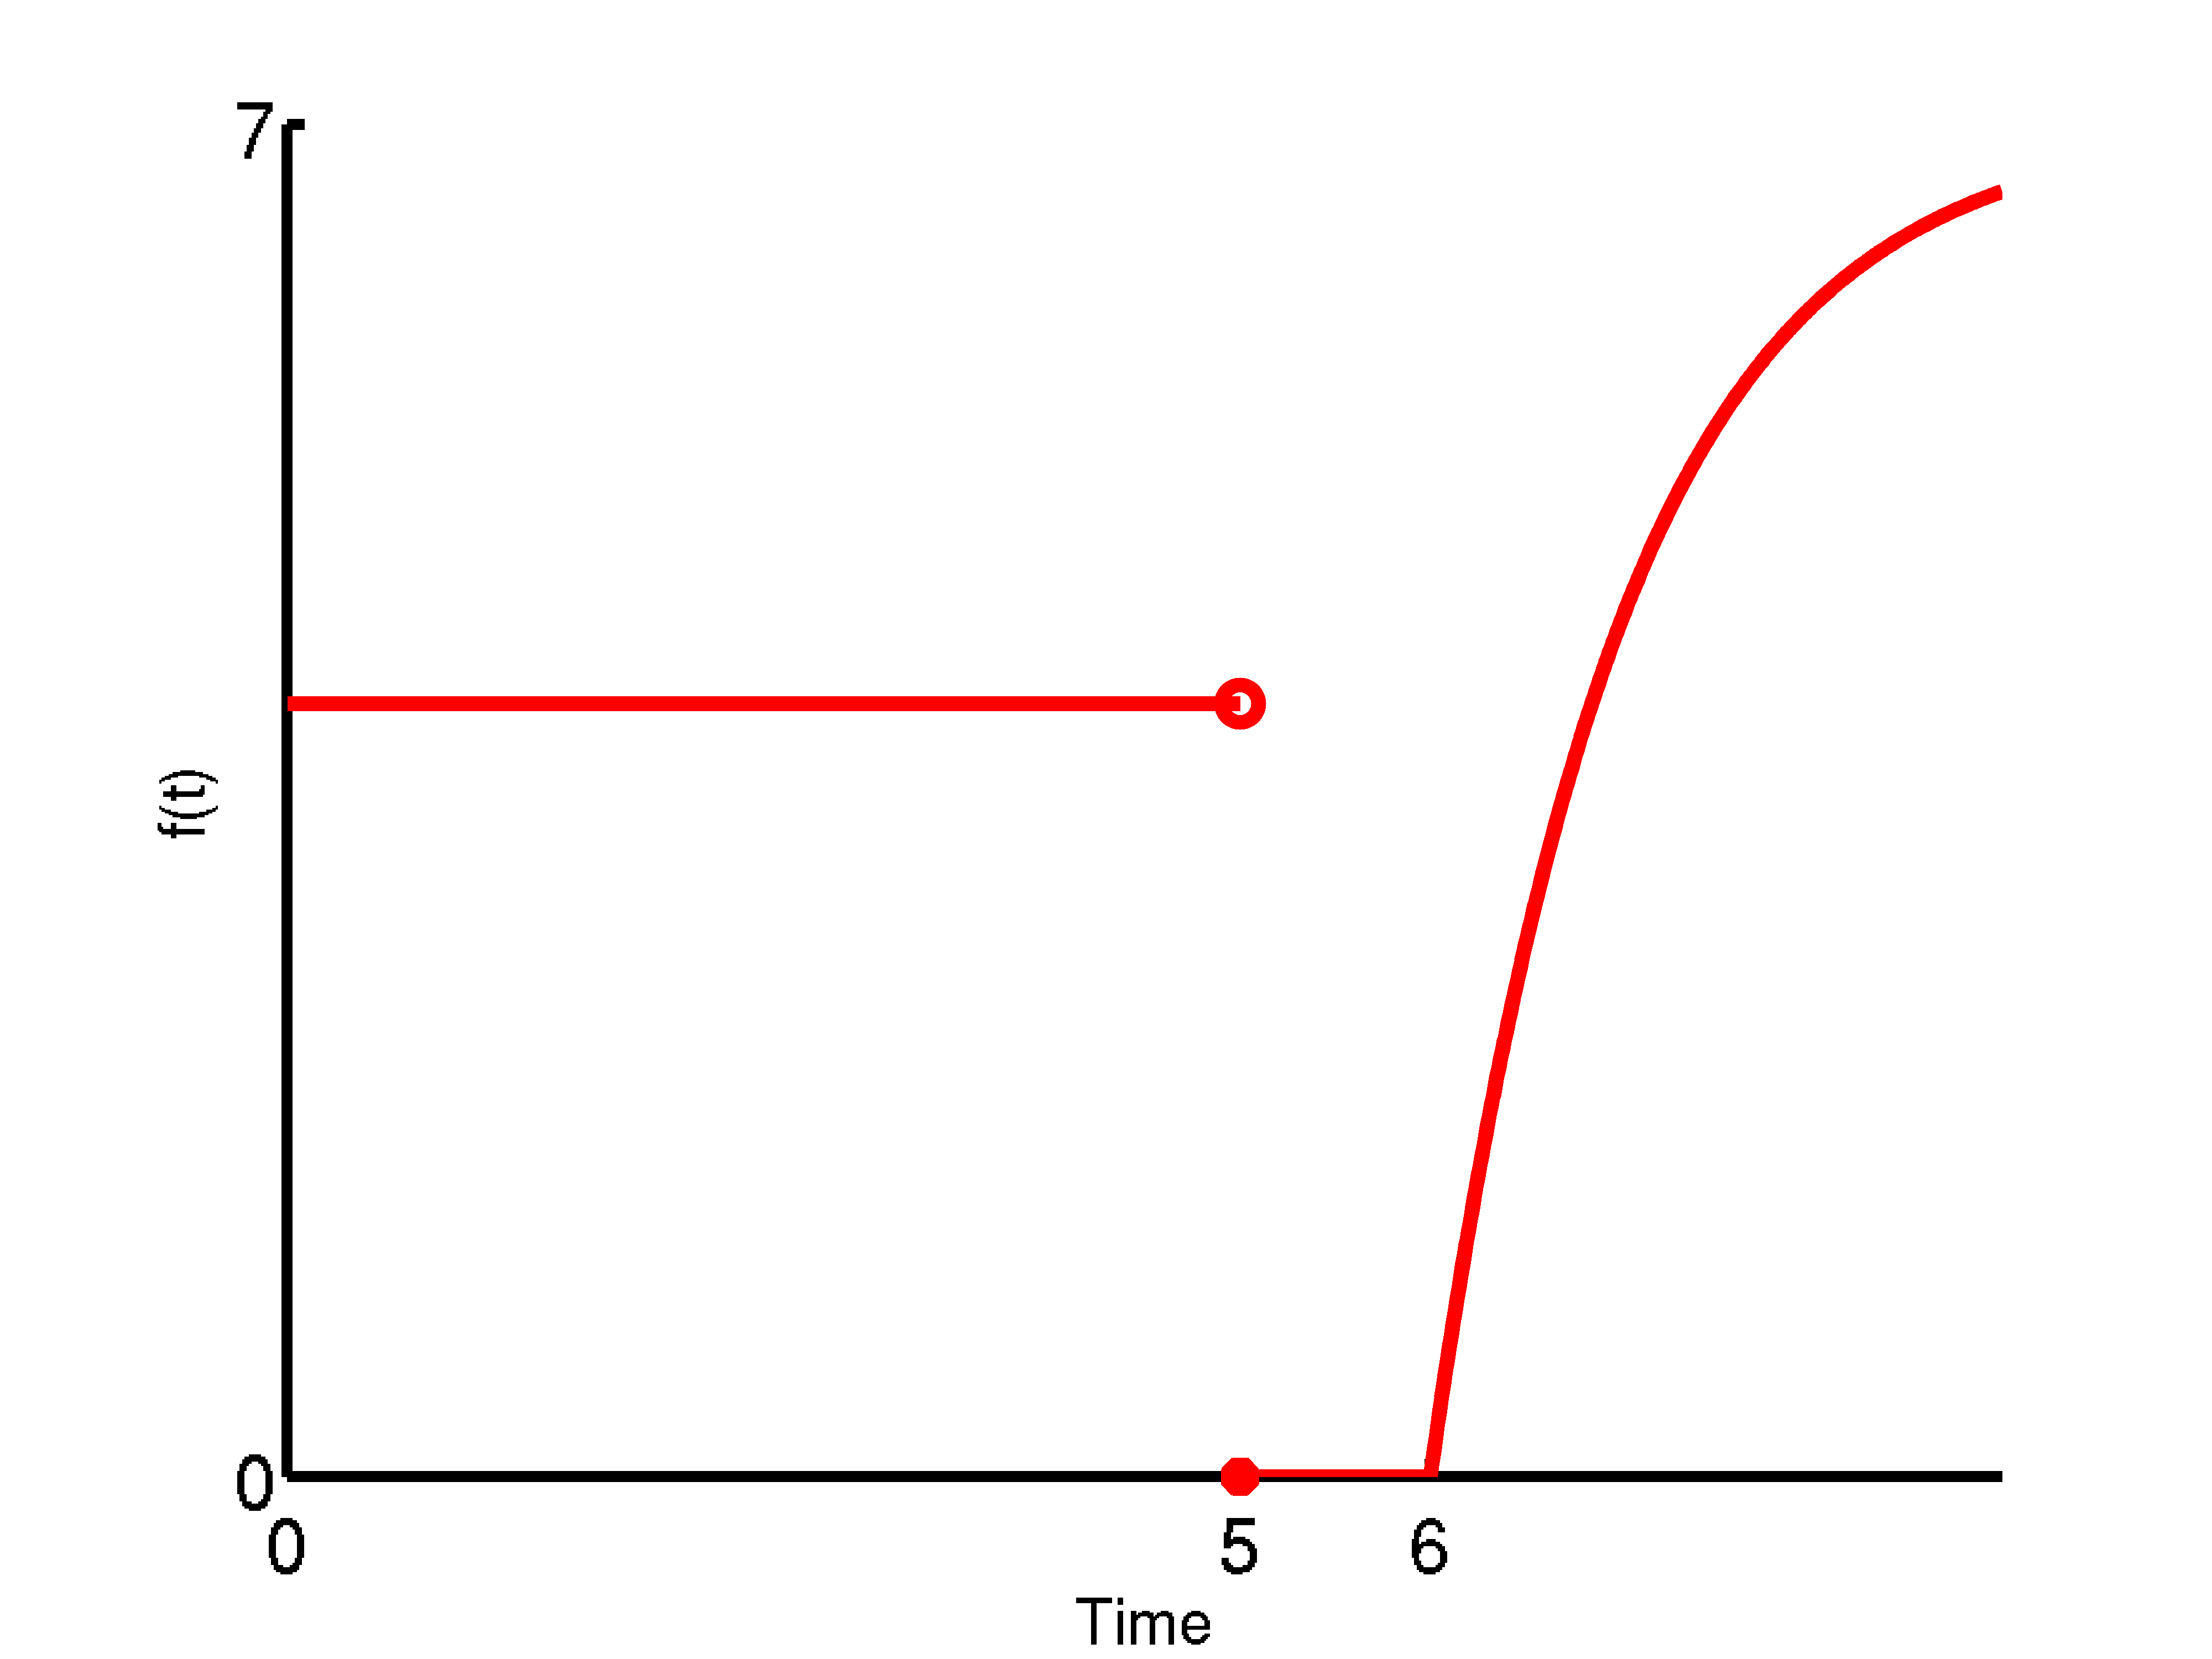
\includegraphics[width=5cm]{img/stepEx6}}

  \begin{eqnarray*}
      f(t) & = & 
      \left\{
        \begin{array}{r@{\hspace{2em}}rcccl}
          7-7e^{-(t-6)} & t & \geq & 6 \\
          0 & 5 & < & t & < & 6 \\
          4 & t & \leq 5 
        \end{array}
      \right.
  \end{eqnarray*}

  \uncover<2->
  {
    \begin{eqnarray*}
      f(t) & = & 4 - 4\cdot\mathrm{step}(t-5) + \lp 7-7e^{-(t-6)}\rp\cdot\mathrm{step}(t-6).
    \end{eqnarray*}
  }


\end{frame}


\subsection{The Laplace Transform of the Unit Step Function}

\begin{frame}
  \frametitle{The Laplace Transform of the Unit Step Function}

  \begin{eqnarray*}
    \laplace{f(\redText{t-a})\mathrm{step(\redText{t-a})}} & = & 
           \int^\infty_0 f(\redText{t-a})\mathrm{step(\redText{t-a})} ~ e^{-st} ~ dt, \\
    & = &  \int^\infty_{\fuchsiaText{a}} f(\redText{t-a}) e^{-st} ~ dt, \\
    & = & \int^\infty_{\fuchsiaText{a}} f(\redText{t-a}) e^{-s(\redText{t-a}+a)} ~ dt, \\
    & = & \int^\infty_{\fuchsiaText{a}} f(\redText{t-a}) e^{-s(\redText{t-a})}\blueText{e^{-as}} ~ dt, \\
    & = & \blueText{e^{-as}} \int^\infty_{\fuchsiaText{a}} f(\redText{t-a}) e^{-s(\redText{t-a})} ~ dt, \\
    & = & \blueText{e^{-as}} \int^\infty_0 f(u) e^{-su} ~ du, \\
    & = & \blueText{e^{-as}} \laplace{f} \\
  \end{eqnarray*}

\end{frame}


\begin{frame}
  \frametitle{Example}

  \begin{eqnarray*}
    \laplace{(t-4)^6\cdot\mathrm{step}(t-4)} & = & e^{-4s}\frac{6!}{s^7}.
  \end{eqnarray*}


\end{frame}


\begin{frame}
  \frametitle{Example}

  \begin{eqnarray*}
    \laplace{\cos\lp 4(t-\pi)\rp\cdot\mathrm{step}(t-\pi)} & = & 
    e^{-\pi s}\laplace{\cos(4t)}, \\
    & = & e^{-\pi s} \frac{s}{s^2+16}.
  \end{eqnarray*}

\end{frame}



\begin{frame}
  \frametitle{Example}

  \begin{eqnarray*}
    \laplace{f} & = & e^{-2s}\frac{1}{(s-4)^2}.
  \end{eqnarray*}

  \only<2->{%
    If 
    \begin{eqnarray*}
      \laplace{g} & = & \frac{1}{(s-4)^2},
    \end{eqnarray*}
    then $g=te^{4t}$.

    Which means that
    \begin{eqnarray*}
      \laplace{f} & = & e^{-2s}\frac{1}{(s-4)^2}, \\
      \Rightarrow f & = & (t-2)e^{4(t-2)} \cdot \mathrm{step}(t-2).
    \end{eqnarray*}
  }

\end{frame}





\begin{frame}
  \frametitle{RC Circuit}

  % Graphic for TeX using PGF
% Title: /home/black/write/class/de/math232-12/ODE-Recitation-Activities/notes/img/stepFunctionCircuit.dia
% Creator: Dia v0.97.2
% CreationDate: Wed Nov 14 15:50:10 2012
% For: black
% \usepackage{tikz}
% The following commands are not supported in PSTricks at present
% We define them conditionally, so when they are implemented,
% this pgf file will use them.
\ifx\du\undefined
  \newlength{\du}
\fi
\setlength{\du}{10\unitlength}
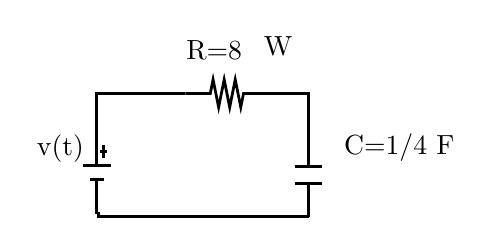
\begin{tikzpicture}
\pgftransformxscale{1.000000}
\pgftransformyscale{-1.000000}
\definecolor{dialinecolor}{rgb}{0.000000, 0.000000, 0.000000}
\pgfsetstrokecolor{dialinecolor}
\definecolor{dialinecolor}{rgb}{1.000000, 1.000000, 1.000000}
\pgfsetfillcolor{dialinecolor}
\pgfsetlinewidth{0.100000\du}
\pgfsetdash{}{0pt}
\pgfsetdash{}{0pt}
\pgfsetbuttcap
\pgfsetmiterjoin
\pgfsetlinewidth{0.100000\du}
\pgfsetbuttcap
\pgfsetmiterjoin
\pgfsetdash{}{0pt}
\definecolor{dialinecolor}{rgb}{0.000000, 0.000000, 0.000000}
\pgfsetstrokecolor{dialinecolor}
\draw (4.550000\du,10.750000\du)--(4.550000\du,12.000000\du);
\pgfsetbuttcap
\pgfsetmiterjoin
\pgfsetdash{}{0pt}
\definecolor{dialinecolor}{rgb}{0.000000, 0.000000, 0.000000}
\pgfsetstrokecolor{dialinecolor}
\draw (4.050000\du,12.000000\du)--(5.050000\du,12.000000\du);
\pgfsetbuttcap
\pgfsetmiterjoin
\pgfsetdash{}{0pt}
\definecolor{dialinecolor}{rgb}{0.000000, 0.000000, 0.000000}
\pgfsetstrokecolor{dialinecolor}
\draw (4.300000\du,12.500000\du)--(4.800000\du,12.500000\du);
\pgfsetbuttcap
\pgfsetmiterjoin
\pgfsetdash{}{0pt}
\definecolor{dialinecolor}{rgb}{0.000000, 0.000000, 0.000000}
\pgfsetstrokecolor{dialinecolor}
\draw (4.800000\du,11.250000\du)--(4.800000\du,11.750000\du);
\pgfsetbuttcap
\pgfsetmiterjoin
\pgfsetdash{}{0pt}
\definecolor{dialinecolor}{rgb}{0.000000, 0.000000, 0.000000}
\pgfsetstrokecolor{dialinecolor}
\draw (4.675000\du,11.500000\du)--(4.925000\du,11.500000\du);
\pgfsetbuttcap
\pgfsetmiterjoin
\pgfsetdash{}{0pt}
\definecolor{dialinecolor}{rgb}{0.000000, 0.000000, 0.000000}
\pgfsetstrokecolor{dialinecolor}
\draw (4.550000\du,12.500000\du)--(4.550000\du,13.750000\du);
\pgfsetlinewidth{0.100000\du}
\pgfsetdash{}{0pt}
\pgfsetdash{}{0pt}
\pgfsetbuttcap
\pgfsetmiterjoin
\pgfsetlinewidth{0.100000\du}
\pgfsetbuttcap
\pgfsetmiterjoin
\pgfsetdash{}{0pt}
\definecolor{dialinecolor}{rgb}{0.000000, 0.000000, 0.000000}
\pgfsetstrokecolor{dialinecolor}
\draw (7.750000\du,9.400000\du)--(8.650000\du,9.400000\du)--(8.750000\du,8.900000\du)--(8.950000\du,9.900000\du)--(9.150000\du,8.900000\du)--(9.350000\du,9.900000\du)--(9.550000\du,8.900000\du)--(9.750000\du,9.900000\du)--(9.850000\du,9.400000\du)--(10.750000\du,9.400000\du);
\pgfsetlinewidth{0.100000\du}
\pgfsetdash{}{0pt}
\pgfsetdash{}{0pt}
\pgfsetbuttcap
\pgfsetmiterjoin
\pgfsetlinewidth{0.100000\du}
\pgfsetbuttcap
\pgfsetmiterjoin
\pgfsetdash{}{0pt}
\definecolor{dialinecolor}{rgb}{0.000000, 0.000000, 0.000000}
\pgfsetstrokecolor{dialinecolor}
\draw (12.200000\du,10.850000\du)--(12.200000\du,12.050000\du);
\pgfsetbuttcap
\pgfsetmiterjoin
\pgfsetdash{}{0pt}
\definecolor{dialinecolor}{rgb}{0.000000, 0.000000, 0.000000}
\pgfsetstrokecolor{dialinecolor}
\draw (11.700000\du,12.050000\du)--(12.700000\du,12.050000\du);
\pgfsetbuttcap
\pgfsetmiterjoin
\pgfsetdash{}{0pt}
\definecolor{dialinecolor}{rgb}{0.000000, 0.000000, 0.000000}
\pgfsetstrokecolor{dialinecolor}
\draw (11.700000\du,12.650000\du)--(12.700000\du,12.650000\du);
\pgfsetbuttcap
\pgfsetmiterjoin
\pgfsetdash{}{0pt}
\definecolor{dialinecolor}{rgb}{0.000000, 0.000000, 0.000000}
\pgfsetstrokecolor{dialinecolor}
\draw (12.200000\du,12.650000\du)--(12.200000\du,13.850000\du);
\pgfsetlinewidth{0.100000\du}
\pgfsetdash{}{0pt}
\pgfsetdash{}{0pt}
\pgfsetmiterjoin
\pgfsetbuttcap
{
\definecolor{dialinecolor}{rgb}{0.000000, 0.000000, 0.000000}
\pgfsetfillcolor{dialinecolor}
% was here!!!
{\pgfsetcornersarced{\pgfpoint{0.000000\du}{0.000000\du}}\definecolor{dialinecolor}{rgb}{0.000000, 0.000000, 0.000000}
\pgfsetstrokecolor{dialinecolor}
\draw (4.550000\du,10.750000\du)--(4.550000\du,10.750000\du)--(4.550000\du,9.400000\du)--(7.750000\du,9.400000\du);
}}
\pgfsetlinewidth{0.100000\du}
\pgfsetdash{}{0pt}
\pgfsetdash{}{0pt}
\pgfsetmiterjoin
\pgfsetbuttcap
{
\definecolor{dialinecolor}{rgb}{0.000000, 0.000000, 0.000000}
\pgfsetfillcolor{dialinecolor}
% was here!!!
{\pgfsetcornersarced{\pgfpoint{0.000000\du}{0.000000\du}}\definecolor{dialinecolor}{rgb}{0.000000, 0.000000, 0.000000}
\pgfsetstrokecolor{dialinecolor}
\draw (12.200000\du,10.850000\du)--(12.200000\du,10.850000\du)--(12.200000\du,9.400000\du)--(10.750000\du,9.400000\du);
}}
\pgfsetlinewidth{0.100000\du}
\pgfsetdash{}{0pt}
\pgfsetdash{}{0pt}
\pgfsetmiterjoin
\pgfsetbuttcap
{
\definecolor{dialinecolor}{rgb}{0.000000, 0.000000, 0.000000}
\pgfsetfillcolor{dialinecolor}
% was here!!!
{\pgfsetcornersarced{\pgfpoint{0.000000\du}{0.000000\du}}\definecolor{dialinecolor}{rgb}{0.000000, 0.000000, 0.000000}
\pgfsetstrokecolor{dialinecolor}
\draw (12.200000\du,13.850000\du)--(4.600000\du,13.850000\du)--(4.600000\du,13.750000\du)--(4.550000\du,13.750000\du);
}}
% setfont left to latex
\definecolor{dialinecolor}{rgb}{0.000000, 0.000000, 0.000000}
\pgfsetstrokecolor{dialinecolor}
\node[anchor=west] at (2.000000\du,11.400000\du){v(t)};
% setfont left to latex
\definecolor{dialinecolor}{rgb}{0.000000, 0.000000, 0.000000}
\pgfsetstrokecolor{dialinecolor}
\node[anchor=west] at (7.400000\du,7.850000\du){R=8};
% setfont left to latex
\definecolor{dialinecolor}{rgb}{0.000000, 0.000000, 0.000000}
\pgfsetstrokecolor{dialinecolor}
\node[anchor=west] at (13.100000\du,11.350000\du){C=1/4 F};
% setfont left to latex
\definecolor{dialinecolor}{rgb}{0.000000, 0.000000, 0.000000}
\pgfsetstrokecolor{dialinecolor}
\node[anchor=west] at (8.050000\du,7.550000\du){};
% setfont left to latex
\definecolor{dialinecolor}{rgb}{0.000000, 0.000000, 0.000000}
\pgfsetstrokecolor{dialinecolor}
\node[anchor=west] at (10.200000\du,7.700000\du){W};
% setfont left to latex
\definecolor{dialinecolor}{rgb}{0.000000, 0.000000, 0.000000}
\pgfsetstrokecolor{dialinecolor}
\node[anchor=west] at (10.650000\du,8.100000\du){};
% setfont left to latex
\definecolor{dialinecolor}{rgb}{0.000000, 0.000000, 0.000000}
\pgfsetstrokecolor{dialinecolor}
\node[anchor=west] at (8.250000\du,7.450000\du){};
% setfont left to latex
\definecolor{dialinecolor}{rgb}{0.000000, 0.000000, 0.000000}
\pgfsetstrokecolor{dialinecolor}
\node[anchor=west] at (10.650000\du,8.300000\du){};
\end{tikzpicture}
    


  \begin{eqnarray*}
    8q' + 4q & = & v(t), \\
    q(0) & = & 0, \\
    v(t) & = & 
    \left\{
      \begin{array}{r@{\hspace{2em}}rcl}
        0 & t & \geq & 6 \\
        2 & t & < & 6
      \end{array}
    \right.
  \end{eqnarray*}

  \uncover<2->
  {
    \begin{eqnarray*}
      8q' + 4q & = & 2 - 2 \cdot \mathrm{step}(t-6).
    \end{eqnarray*}
        
  }

\end{frame}


\begin{frame}
  \frametitle{Take the Laplace Transform}

  \begin{eqnarray*}
    8\lp -q(0) + s \laplace{q} \rp + 4 \laplace{q} & = & \frac{2}{s} -
    \frac{2}{s} e^{-6s}.
  \end{eqnarray*}

  \uncover<2->
  {
    \begin{eqnarray*}
      \laplace{q} & = & \blueText{\frac{1/2}{s(2s+1)}} \redText{- \frac{1/2}{s(2s+1)} e^{-6s}}, \\
      & = & \blueText{\half \frac{1}{s} - \half \frac{1}{s+\half}}
      \redText{- \half \frac{1}{s} e^{-6s} + \half \frac{1}{s+\half} e^{-6s}}.
    \end{eqnarray*}
  }

  \uncover<3->
  {
    \begin{eqnarray*}
      q & = & \blueText{\half - \half e^{-t/2}} \\
      & & \redText{- \half\cdot\mathrm{step}(t-6)
                   + \half e^{-(t-6)/2}\cdot\mathrm{step}(t-6)}.
    \end{eqnarray*}
  }


\end{frame}




% LocalWords:  Clarkson pausesection hideothersubsections rcl rr rcccl dt
